% This is samplepaper.tex, a sample chapter demonstrating the
% LLNCS macro package for Springer Computer Science proceedings;
% Version 2.21 of 2022/01/12
%
\documentclass[runningheads]{llncs}
%
\usepackage{adjustbox}
\usepackage[T1]{fontenc}
% Import additional packages in the preamble file, before hyperref
%
% --- inline annotations
%
%hack to fix everyshi.sty: https://tex.stackexchange.com/questions/398223/tikz-gives-error-command-everyshipouthook-already-defined
\makeatletter
\@namedef{ver@everyshi.sty}{}
\makeatother
\usepackage{tikz}

% Include other packages here, before hyperref.
\usepackage{graphicx}
\usepackage{amsmath}
\usepackage{amssymb}
\usepackage{booktabs}
\usepackage{multirow}
\usepackage[boldmath]{numprint}
\usepackage{multicol}

% \newcommand{\etal}{\textit{et al}.}
% \newcommand{\ie}{\textit{i}.\textit{e}.}
% \newcommand{\eg}{\textit{e}.\textit{g}.}
\newcommand{\keypoint}[1]{\vspace{0.1cm}\noindent\textbf{#1}\quad}


\newcommand{\tobacco}{\textsl{Tobacco-3482}}
\newcommand{\rvl}{\textsl{RVL-CDIP}}
\newcommand{\rvlone}{\textsl{RVL-CDIP$_{1k}$}}
\newcommand{\tablebank}{\textsl{TableBank}}
\newcommand{\doclaynet}{\textsl{DocLayNet}}
\newcommand{\prima}{\textsl{PRImA}}

%metrics
\newcommand{\ECE}{$\mathrm{ECE}$}
\newcommand{\NLL}{$\mathrm{NLL}$}
\newcommand{\BS}{$\mathrm{BS}$}
\newcommand{\EAURC}{$\mathrm{E-AURC}$}
\newcommand{\AUROC}{$\mathrm{AUROC}$}
\newcommand{\AURC}{$\mathrm{AURC}$}
\newcommand{\ANLS}{$\mathrm{ANLS}$}

% colors
\colorlet{darkgreen}{green!60!black!80!}
\colorlet{darkorange}{orange!60!black!80!}
\colorlet{purple}{red!80!green!20!blue!60!}
\colorlet{darkpurple}{red!90!green!20!blue!90!}

\definecolor{OliveGreen}{cmyk}{0.64,0,0.95,0.40}
\definecolor{ForestGreen}{RGB}{34,139,34}
% Reviews
\newcommand{\smy}[1]
{\leavevmode#1}%{{\leavevmode\color{orange}#1}}
\newcommand{\sbs}[1]{\leavevmode#1}%{{\leavevmode\color{blue}#1}}
\newcommand{\ayb}[1]{\leavevmode#1}%{{\leavevmode\color{brown}#1}}
\newcommand{\jvl}[1]{\leavevmode#1}%{{\leavevmode\color{darkpurple}#1}}
\newcommand{\commentout}[1]{\ignorespaces}

% Drafting
\setlength {\marginparwidth }{2cm}
\usepackage[colorinlistoftodos,prependcaption]{todonotes} %,textsize=tiny
\usepackage{xargs}  % Use more than one optional parameter in new command
\newcommandx{\draft}[2][1=]{\todo[linecolor=ForestGreen,backgroundcolor=ForestGreen!25,bordercolor=ForestGreen,inline,caption={},#1]{#2}}
\newcommandx{\exactcopy}[2][1=]{\todo[linecolor=darkorange,backgroundcolor=darkorange!25,bordercolor=darkorange!50,inline,#1,noprepend,caption={}]{\small #2}}


%sectioning
\newcommand{\etal}{\textit{et al}.}
\newcommand{\ie}{\textit{i}.\textit{e}.}
\newcommand{\eg}{\textit{e}.\textit{g}.,}
\makeatletter
\DeclareRobustCommand\onedot{\futurelet\@let@token\@onedot}
\def\@onedot{\ifx\@let@token.\else.\null\fi\xspace}

\def\eg{\emph{e.g}\onedot, } \def\Eg{\emph{E.g}\onedot, }
\def\ie{\emph{i.e}\onedot, } \def\Ie{\emph{I.e}\onedot, }
\def\cf{\emph{cf}\onedot} \def\Cf{\emph{Cf}\onedot}
\def\etc{\emph{etc}\onedot} \def\vs{\emph{vs}\onedot}
\def\wrt{w.r.t\onedot} \def\dof{d.o.f\onedot}
\def\iid{i.i.d\onedot} \def\wolog{w.l.o.g\onedot}
\def\etal{\emph{et al}\onedot}
\makeatother

 
% marks
\usepackage{amssymb}
\newcommand{\bluecheck}{{\color{blue}\checkmark}}
\usepackage{pifont}% http://ctan.org/pkg/pifont
\newcommand{\redmark}{{\color{red}\ding{55}}}%

%abbreviations and math
\DeclareMathOperator*{\argmax}{argmax} % thin space, limits underneath in displays
\usepackage{mathtools}
\DeclareMathOperator{\Prob}{\mathbb{P}}
\DeclareMathOperator{\Exp}{\mathbb{E}}
\DeclareMathOperator{\Var}{\mathbb{V}}
\DeclareMathOperator{\Cov}{\mathbb{C}}
\DeclareMathOperator{\Ber}{Ber}
\DeclareMathOperator*{\esssup}{ess\,sup}
\newcommand{\norm}[1]{\left\lVert#1\right\rVert}

% For pseudo algorithms
\usepackage[linesnumbered,ruled,vlined]{algorithm2e}
\SetKwComment{Comment}{$\triangleright$\ }{}
\newcommand\mycommfont[1]{\footnotesize\ttfamily\textcolor{blue}{#1}}
\SetCommentSty{mycommfont}

\newcommand*{\xml}[1]{\texttt{<#1>}}
\newcommand*{\xmlend}[1]{\texttt{</#1>}}


\usepackage{enumitem} %dotted lines

\usepackage{arydshln} %dotted lines
\setlength\dashlinedash{0.2pt}
\setlength\dashlinegap{1.5pt}
\setlength\arrayrulewidth{0.3pt}

%captionsetup 

%hange here
\makeatletter
\renewcommand\paragraph{\@startsection{paragraph}{4}{\z@}%
                                    {3.25ex \@plus1ex \@minus.2ex}%
                                    {-1em}%
                                    {\normalfont\normalsize\bfseries}}
\makeatother


% PUT ANYTHING BEFORE THIS except hyperref and cleverref
\definecolor{cvprblue}{rgb}{0.21,0.49,0.74}
\usepackage[pagebackref,breaklinks,colorlinks,citecolor=cvprblue]{hyperref}


% Support for easy cross-referencing
\usepackage[nameinlink,capitalize,noabbrev]{cleveref}
\crefname{section}{Sec.}{Secs.}
\Crefname{section}{Section}{Sections}
\Crefname{table}{Table}{Tables}
\crefname{table}{Tab.}{Tabs.}



\usepackage[square]{natbib}

\usepackage{graphicx} % Required for inserting images

\usepackage{caption}

\usepackage{floatrow} 


% \captionsetup{belowskip=0pt}
% \captionsetup{aboveskip=0pt}


\begin{document}

%\captionsetup{format=plain, font=small, labelfont=bf}
\captionsetup{
  %justification=centering,
  singlelinecheck=false,
  font=small,labelfont=bf,labelsep=space,belowskip=10pt,aboveskip=10pt}

\floatsetup[table]{capposition=top}
\floatsetup[figure]{capposition=bottom}


\newlength{\parskiplength}
\setlength{\parskiplength}{8pt}

%\setlength{\floatsep}{\parskiplength}
\setlength{\textfloatsep}{\parskiplength}
\setlength{\intextsep}{\parskiplength}

% \onecolumn
% \setcounter{tocdepth}{5}
% \tableofcontents

% \clearpage
% \setcounter{page}{1}
% \twocolumn

%%%%%%%%% TITLE - PLEASE UPDATE

%"DistilDoc: Accelerating Visually-Rich Document Understanding using Knowledge Distillation"

\title{\texttt{DistilDoc}: Knowledge Distillation for Visually-Rich Document Applications} %or tasks?
%DistilDoc: What can Knowledge Distillation do for Visual Documents Representations?




\author{
  \small Jordy Van Landeghem\inst{1,2}, 
  \small Subhajit Maity \inst{}, 
  \small Ayan Banerjee\inst{3}, 
  \small Matthew Blaschko\inst{1}, 
  \small Sien Moens\inst{1}, 
  \small Josep Llados\inst{3}, 
  \small Sanket Biswas\inst{3}
}

\institute{\footnotesize KU Leuven 
    %\and \email{firstname.lastname@student.kuleuven.be}
\and
\footnotesize Contract.fit \quad 
\email{jordy@contract.fit}
\and
\footnotesize Computer Vision Center, Universitat Autònoma de Barcelona
}

\maketitle

%%%%%%%%% ABSTRACT

\begin{abstract}
\jvl{
This work explores knowledge distillation (KD) for visually-rich document (VRD) applications such as document layout analysis (DLA) and document image classification (DIC). While VRD research is dependent on increasingly sophisticated and cumbersome models, the field has neglected to study efficiency via model compression. Here, we 
design a KD experimentation methodology\footnote{Code and Datasets are linked in \Cref{supp:code_and_datasets}}
for more lean, performant models on document understanding (DU) tasks that are integral within larger task pipelines.
\\
We carefully selected KD strategies (\textsl{response-based, feature-based}) for distilling knowledge to and from backbones with different architectures (\textsl{ResNet, ViT, DiT}) and capacities (\textsl{base-small-tiny}).
We study what affects the teacher-student knowledge gap and find that some methods (tuned \textsl{vanilla KD}, \textsl{MSE}, \textsl{SimKD} with an apt projector) can consistently outperform supervised student training. Furthermore, we design a downstream task setup to evaluate the robustness of distilled DLA models on zero-shot layout-aware document visual question answering (DocVQA). \\
DLA-KD experiments result in a large mAP knowledge gap, which unpredictably translates to downstream robustness, accentuating the need to further explore how to efficiently obtain more semantic document layout awareness.
}

%We design two downstream task setups where the output of distilled DLA models will 

%In ablation, we employ linear probes to investigate cross-architecture and cross-task distillation in an effort to better understand the impact of KD on visual document representations.
   % Knowledge distillation had been one of the emerging fields of research in computer vision and deep learning communities and is used in abundance for improving efficiency via model compression. However, document research, largely dependent on novel strategies and sophisticated models from the vision community, has not delved much into knowledge distillation. 
   % Here, we explore the scope of knowledge distillation in document research, as well as what benefits it can bring along, if any. We carefully selected a multitude of knowledge distillation strategies, that work differently in terms of working principles, for distilling knowledge to and from backbones with different architectures. We compare their performances with a fully supervised baseline showing that the knowledge distillation strategies mostly perform at par with supervision if not outperform. We also analyze how knowledge distillation impacts generalization on different document tasks and observed that none of the distillation strategies fully dominate over the other terms of performance or generalization and have their unique advantages and disadvantages.
\end{abstract}


% We compare their performance with a fully supervised baseline showing that the knowledge distillation strategies mostly perform at par with supervision if not outperform. We also analyze how knowledge distillation impacts generalization on different document tasks and observed that none of the distillation strategies fully dominate over the other terms of performance or generalization and have their unique advantages and disadvantages.
%region-based analysis -> better and leaner DLA models will help to more efficiently model long documents, now the models are of the same size 


%%%%%%%%% BODY TEXT
\section{Introduction}
\label{sec:intro}

Visually-rich Document Understanding (DU) has attracted increasing interest over the last few years.
It involves multiple tasks such as document image classification (DIC) ~\cite{kang2014convolutional, harley2015evaluation, jain2019multimodal, liu2021document}, key information extraction (KIE)~\cite{liao2023doctr,luo2023geolayoutlm, simsa2023docile, jaume2019funsd, stanislawek2021kleister}, document layout analysis (DLA)~\cite{binmakhashen2019document, pfitzmann2022doclaynet, da2023vision, zhong2019publaynet, biswas2021beyond} and document visual question answering (VQA)~\cite{mathew2021docvqa, ding2022v, mathew2022infographicvqa, tito2021icdar}.
Current state-of-the-art (SOTA) DU models~\cite{huang2022layoutlmv3,gu2021unidoc} solve the task by using modern OCR engines to read the text and then combine them with spatial features to predict the page layout and structure. However, these multimodal architectures come with the following drawbacks: 1) They rely primarily on Large Language Models (LLMs) \cite{zhao2023survey} % (\eg BERT~\cite{devlin2018bert} or GPT~\cite{brown2020language}) 
pretrained on millions of samples which depend more on OCR text quality than visual features/document structure 2) can be computationally heavier due to the need to process and fuse information from different modalities 3) may perform poorly in domains with poor OCR results or on low-resource languages.

Therefore, this work focuses on single-modality, vision-only architectures that can be fine-tuned for handling VRDs in tasks involving understanding visual-layout semantics such as tables, titles, paragraphs, figures, \etc. \\
DLA is a useful preliminary step in a document processing workflow~\cite{binmakhashen2019document, da2023vision}, holding the key to enhancing practical downstream DU tasks such as DIC, KIE, and VQA. DLA can impart \textit{logical layout} structure, beyond \textit{geometric layout} from OCR \cite{haralick1994document}, and structured context to the document, to enable more accurate content extraction and interpretation. A recent DU competition~\cite{VanLandeghem2023icdar} has pleaded to bridge the gap between DLA and DocVQA by introducing layout-navigating or multi-region questions.

%for given tasks, it might be sensical to focus on a specific modality-only
To handle the computational demand of modality/task-specific models, knowledge distillation (KD) \cite{ba2014deep,hinton2015distilling,romero2014fitnets,gou2021knowledge} can prove an effective approach to obtain efficient modules for later re-use in enriching LLM document inputs. Teacher model compression has the potential to make student models that improve over direct fine-tuning, also making them practical for deployment with resource-constrained devices or for faster real-time inference.
The field of Document AI ~\cite{cui2021document} is engaged with representing and understanding VRDs, but thus far has not explored KD-based model compression for improved efficiency and uncertainty estimation \cite{galil2023can}.

This work investigates the potential of enriching VRDs with logical layout structure derived from effective DLA model compression using KD methods to practically and efficiently improve downstream DU applications.
The nature of the (document) dataset has a major impact on the KD process \cite{stanton2021does}, which required motivated choices (regarding dataset usage \cite{pfitzmann2022doclaynet,
    antonacopoulos2009realistic,
    harley2015evaluation}, architectures, weight initialization \cite{li2022dit}, KD methods~\cite{SimKD, he2021distilling, chen2021distilling, zhang2020distilling, hsieh2023distilling,hinton2015distilling}, evaluation, downstream procedure \cite{wang2023layout}, \etc) in designing our novel experimental methodology of KD benchmarking for DU tasks (DIC, DLA). This allows us to investigate aspects affecting teacher-student knowledge/capacity/initialization gaps.

\noindent The key contributions of the paper are twofold:
\begin{enumerate}
    [label=\Roman*.,leftmargin=2\parindent]
    \item  We are the first to design, apply, and open-source an experimental methodology for comprehensively benchmarking KD-based model compression on DU tasks involving VRDs (DIC and DLA).
    \item  We design a novel evaluation procedure based on the downstream task of zero-shot layout-aware DocVQA to quantify the robustness of distilled DLA models.
\end{enumerate}

\noindent Nevertheless, our key contributions go beyond mere KD-based compression benchmarking, promoting logical layout analysis over geometric layout to enhance the generalization of DU models toward unseen documents with diverse and complex layouts, as demonstrated in \Cref{fig:new-hero}.

\section{Related Work}

\sbs{\paragraph{Efficiency and Model Compression}

    Efficiency through model compression is gaining relevance with the increasing parameter size and complexity of models such as LLMs \cite{zhu2023survey}. Although KD is a prominent technique for model compression, several alternative approaches are worth mentioning.
    \textit{Quantization} has been recently re-discovered in the context of LLMs with LoRA~\cite{hu2021lora} and Q-LoRA~\cite{dettmers2023qlora} that achieves substantial model compression with minimal accuracy degradation. Advances have been made also in vision-and-language~\cite{cao2017deep, yuan2020central} and more recently for vision transformer (ViT) training~\cite{li2023vit}. However, its effectiveness also depends on some key factors, including the model architecture, data type, bit-width, and the training recipes employed. In this direction, \textit{neural architecture search} (NAS) became an important field of study~\cite{cai2018efficient, liu2018progressive, liu2017hierarchical, pham2018efficient}. Popular alternatives include \textit{model weight pruning}~\cite{zhu2017prune, liu2018rethinking, gao2021network} that benefits strongly from
    %from requires to be used judiciously and in conjunction 
    joint usage with other efficiency and model compression techniques;  \textit{adaptive inference} with multi-exit architectures~\cite{xing2020early, zhou2020bert}, which are promising yet highly dependent on early exit network design and uncertainty estimation.
    %impactful lately, especially in adaptive inference stage, where the model could decide whether to continue processing the input or stop early based on the confidence of the model predictions. However, design choices of the network remain the key for getting the best out of this strategy. 
    KD-based training ~\cite{phuong2019distillation} complements the aforementioned techniques, leading to potentially more accurate model exits and pruning. Moreover, KD strategies involve overall simpler design choices, depending mostly on the availability of a large teacher model trained on domain data of interest. Therefore, we prioritize KD-based model compression and efficiency for practical DU applications.

    %In this context, \textit{knowledge distillation} strategies have a much simpler design choice with the availability of a large teacher model and could help in better interpretability on how distilled predictions (student) could match the assigned softer targets (teacher). In this work, we investigated the utility of KD strategies towards achieving model compression and efficiency for practical DU applications.

    % Compress a large model for efficient deployment.
    % Transfer knowledge from a pretrained model to a smaller one.
    % Improve generalization on small datasets.
    % Create an ensemble of models from multiple teachers.
    % Continuously update a model while retaining past knowledge.
    % Simplify a complex model for better interpretability.
    % These alternatives encompass various strategies, such as efficient architecture design, early exits, quantization, neural architecture search~\cite{cai2018efficient, liu2018progressive, liu2017hierarchical, pham2018efficient}, model weight pruning, and hardware-software co-design. 
}
% 
\paragraph{Knowledge Distillation}


KD strategies can be categorized into three main categories: \textit{response-based} KD~\cite{ba2014deep, hinton2015distilling, aditya2019spatial, mirzadeh2020improved, zhao2022decoupled, yang2023knowledge} seeks to match the final layer predictions of the teacher model; \textit{feature-based} KD~\cite{romero2014fitnets, ahn2019variational, heo2019knowledge,komodakis2017paying, chen2021cross, chen2021distilling} aims to mimic features extracted from intermediate hidden layers of the deep network and \textit{relation-based} KD~\cite{yim2017gift, park2019relational, tian2019contrastive, passalis2020heterogeneous} which exploits the relations between different layers or sampled data points. However, the latter approach is more geared toward pixel-based semantic segmentation tasks. While feature-based KD is more versatile, it is more expensive and harder to implement than soft teacher predictions.
While offline methods~\cite{hinton2015distilling, romero2014fitnets} consider an existing frozen teacher model, online methods~\cite{zhang2018deep, chen2020online} update both student and teacher networks jointly. Self-distillation~\cite{bagherinezhad2018label, zhang2019your} represents a special case of online KD, which employs the same network as both the teacher and student, progressively outperforming the network's performance, albeit disregarding the aim of efficiency.

Our work's scope will be offline KD schemes% (vs. online and self-distillation)
, with a single converged teacher (vs. intermediate checkpoints \cite{wang2022efficient} or ensembles \cite{you2017learning}), single modality inputs (vision only), with three different feature extraction backbones (ResNets, ViT and a self-supervised pretrained document foundation model DiT~\cite{li2022dit}). Our study seeks to extend the empirical utility of KD to popular DU tasks
(DIC \& DLA) with a versatile benchmarking framework to ensure future compatibility, fostering KD-based DU model compression research.


\paragraph{Practical and Efficient Document Understanding}
%Practical and efficient DU: logical layout to the rescue? 
\sbs{ Recent efforts to represent layout and document structure have gained substantial recognition, particularly with the incorporation of structural information into LLMs. The LayoutLM family~\cite{huang2022layoutlmv3, xu2020layoutlm, xu2020layoutlmv2} and GeoLayoutLM~\cite{luo2023geolayoutlm} laid the foundation of using 2D positional information of text (word blocks) tokens obtained from OCR as a \textit{geometric layout} representation for the input. Recent work \cite{shen2022vila} has further enhanced this 2D representation by incorporating text lines or text blocks as layout groups inside the OCR text tokens. \cite{wang2023layout} further experiments with structure-preserving OCR, that uses appropriate spaces and line breaks as an LLM input, thereby improving the ability to capture layout and structural cues for zero-shot DocVQA~\cite{mathew2021docvqa, mathew2022infographicvqa} tasks.
\cite{li2021selfdoc,gu2021unidoc} seek to represent layout as region-level proposal features, representing \textit{logical layout} elements like title, paragraph, figure, tables, \etc) as in the DLA task. To further study the utility of logical layout representations, \cite{wu2022region} addresses asking questions conditioned inside a specific region of a page, improving upon the design of DocVQA that provides too many in-line questions ($>$80\%). More recently, PDFTriage~\cite{saad2023pdftriage} generates a structured metadata representation of born-digital documents, extracting both geometric and logical layout elements like section text, figure captions, headers, and tables for a more precise QA approach.  DUDE~\cite{VanLandeghem2023dude} offers a testing bed for DocVQA on multipage, multi-type documents with varying layouts, including questions conditioned on layout navigation, \eg `\textsl{Which pages have tables?}'.

    Our explorations focus on making the most of the logical layout features obtained from the multi-domain DLA benchmark, DocLayNet~\cite{pfitzmann2022doclaynet}. We build upon the aforementioned advancements and explore how incorporating document structure can enhance the performance of downstream task models, aligning with the trend of enriching LLMs with rich-text prompting and layout-aware representations.}



% While the standard interface for many models is text-in and text-out, recent developments have focused on enriching textual prompts to better capture layout and structural cues. Notable contributions in this direction include the LayoutLM series, SelfDoc, Hi-VILA, and Latin-Prompt, which have sought to connect natural language understanding and document layout analysis. In our study, we build upon these advancements and explore how incorporating structural information can enhance the performance of DIC and DLA models, aligning with the broader trend of enriching language models with rich-text prompting and layout-aware representations.}

% \draft{
%   \begin{itemize}
%     \item Practical DU
%           \begin{itemize}
%             \item Background on document image classification practices (approaches, SOTA; difference between geometric (OCR) and logical layout) 
%             \item Background on document layout analysis practices (approaches, SOTA, downstream)
%             \item The two core tasks tested with KD methods are classification and recognition. Alternative tasks are generation, ranking or regression; which are not considered in this work.
%           \end{itemize}
%   \end{itemize}
% }

% \jvl{
% \draft{
% our exploration only treats logical layout analysis based on DocLayNet (richest document structure scheme available), yet we believe in the future -> DLA vs. document object detection ; split is arbitrary? 


% logical (header-title-body-footer lineitem figure table) versus geometric (text block) layout analysis (Haralick, 1994). 

% 2D position embeddings in LayoutLM / geoLayoutLM incorporate document structure into representation learning

% Selfdoc, unidoc - region-base

% Hi-Vila = geometric (OCR blocks)

% LATIN-prompt puts structure-preserving OCR in the foreground again (this is good LLM input yo) - still geometric only

% PDFtriage: if native then use whatever structure is embedded in the pdf (geometric - logical - metadata attributes); no solution for scanned, hence more rich document structure annotations needed. 

% RegionDocVQA: \cite{wu2022region} asking questions conditioned inside a specific region; criticism on docvqa as a dataset with too many in-line or in-question QA pairs. (give examples) 
% }}


%https://community.openai.com/t/support-for-rich-text-format-prompts-in-chatgpt/388486
%https://dl-acm-org.kuleuven.e-bronnen.be/doi/abs/10.1145/3503161.3548172?casa_token=4d18HlasPA8AAAAA%3AYYM7C_nZkvIJsN-py1H4IffQk5hfJL8ZawIMhXRzUMK8uXYRfzcAD-U0ssyCfw949b3OeFXf_JFw 
%difference between in-line and in-region questions 

\jvl{
    \section{Experimental Setup}\label{sec:exps}

    \begin{figure*}[t]
        \centering
        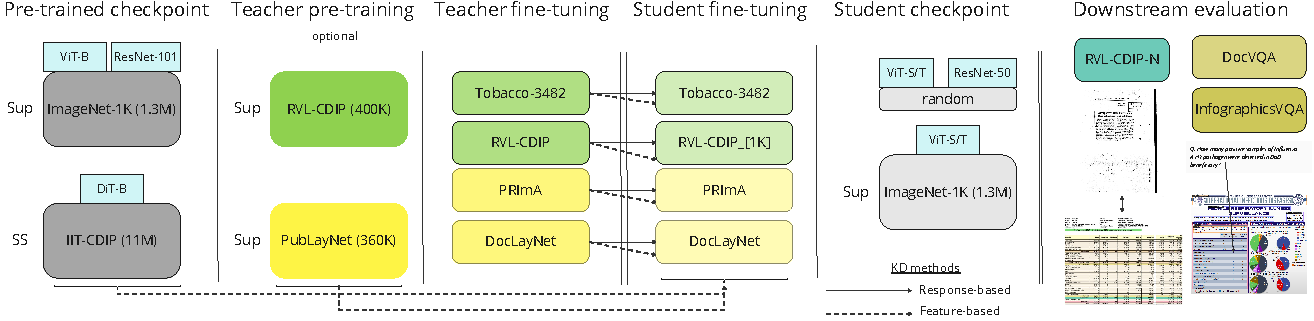
\includegraphics[width=\textwidth]{images/distildoc_v6.pdf}
        \caption{\jvl{Proposed KD experimental methodology with datasets, architectures, and evaluation for DIC and DLA applications. Discussed in detail in \Cref{sec:exps}}}
        \label{fig:backup-hero}
    \end{figure*}

    This Section documents the experimental methodology established in this work (also visualized in \cref{fig:backup-hero}), including datasets, architectures \& backbones for teacher and student models, KD methods, and evaluation metrics for the tasks and distillation effectiveness.
    The goal is to provide a framework for future research on KD for DU tasks and allow pinpoint comparisons on KD aspects such as teacher-student knowledge and capacity gap, teacher-pretraining, student network initialization, \etc
}

\begin{table}[ht]
    \centering
    \caption{Dataset usage for DIC, DLA, and downstream tasks.
        Symbols: P = pretraining, DP = document pretraining, T = teacher training, S = student training, * = subsampling, E = teacher/student evaluation, D: downstream evaluation}
    \begin{tabular}{|l|l|c|c|c|}
        \hline
        \textbf{Dataset}                            & \textbf{Task} & \textbf{Usage} & \textbf{Size} & \textbf{\# Cls} \\ \hline
        ImageNet \cite{deng2009imagenet}            & DIC           & P              & 1.28M         & 1000            \\ \hline
        IIT-CDIP \cite{lewis2006building}           & DIC           & DP,T,S         & 11M           & /               \\ \hline
        \tobacco \cite{kumar2013unsupervised}       & DIC           & T,S,E          & 3482          & 10              \\ \hline
        \rvl \cite{harley2015evaluation}            & DIC           & DP,T,E         & 400K          & 12              \\ \hline
        %MSCOCO \cite{lin2014microsoft}               & DLA           & (P)            & 133K          & 80              \\ \hline
        %PubLayNet \cite{zhong2019publaynet}          & DLA           & (DP,T,S)       & 360K          & 5               \\ \hline
        \prima \cite{antonacopoulos2009realistic}   & DLA           & T,S,E          & 400           & 6               \\ \hline
        \doclaynet \cite{pfitzmann2022doclaynet}    & DLA           & T,S,E          & 80.8K         & 11              \\ \hline \hline
        RVL-CDIP-N \cite{larson2022evaluating}      & DIC           & D              & 1K            & 16              \\ \hline
        SP-DocVQA \cite{tito2021icdar}              & VQA           & D              & 12.8K         & 50K             \\ \hline
        Infographic \cite{mathew2022infographicvqa} & VQA           & D              & 5.5K          & 30K             \\ \hline
        \hline
    \end{tabular}
    \label{tab:DKD-datasets}
\end{table}



\subsection{Datasets}\label{sec:datasets}

\jvl{
    \cref{tab:DKD-datasets} lists all datasets used (in)directly for the experiments. As there is no existing methodology for KD experimentation on the tasks involved, we motivate the design choices:

    \textbf{DIC} We benchmark results on both \tobacco{} (original train-val-test splits 800-200-2482) and \rvl.
    The originally large training size of \rvl{} hinders experimentation (long iteration cycles), which is why we create a subsampled student training set, \rvlone, by randomly selecting 1K images per class.
    By evaluating the full \rvl{} test set, we provide a fair evaluation of the usefulness of KD methods, while avoiding the cumbersomeness of student fine-tuning on such a large dataset.

While \rvl{} is the de facto standard for measuring DIC performance, the literature \cite{larson2023labelnoise,VanLandeghem2024bdpc} has reported several undesirable characteristics such as (near-)duplicates causing substantial overlap between train and test distributions.
    % Without a better alternative existing, we take these points into account when experimenting with KD methods. 
    We complement independently and identically distributed (\textit{i.i.d.}) test set evaluation with benchmarking on RVL-CDIP-N \cite{larson2022evaluating}, which is a covariate shift dataset allowing us to evaluate the robustness of KD methods to domain shift, which is a common problem in real-world applications.
}

\jvl{
    \noindent\textbf{DLA} We benchmark results on \doclaynet{} (reporting evaluation on validation set following common practice) and \prima{}. The former is a large-scale human-annotated dataset with 81K images and 11 categories of logical layout elements, while the latter is a smaller dataset with 400 images and 6 classes. \doclaynet{} contains a wide layout variability with six diverse document types (patents, scientific, legal, reports, tenders) in English. They have been hand-annotated by trained experts, making it the gold standard for DLA. Alternatively, Publaynet~\cite{zhong2019publaynet} or MS-COCO~\cite{lin2014microsoft} benchmarks have been used in pretraining DLA models. However, the former lacks diversity as it only contains documents from the scientific domain while the latter is a more common object detection benchmark for natural scenes.
}

\jvl{
    We consider a mirrored data setup for both tasks, with one larger benchmark dataset (\rvl, \doclaynet) and a smaller, easier dataset (\tobacco, \prima).
    This allows us to compare KD efficacy with more or less accurate teachers over tasks. %getting more insight into teacher-student knowledge gap with in low/high-accuracy regimes
}

\jvl{
    \subsection{Architectures and Backbones}\label{sec:architectures}

    We evaluated three backbone architectures, representing different approaches to the tasks of DIC and DLA.

    \paragraph{Backbones}
    \noindent Residual Network (\textit{ResNet}) \cite{he2016deep}: A supervised pretrained CNN-based architecture that is a staple in image recognition.

    \noindent Vision Transformer (\textit{ViT}) \cite{dosovitskiy2020image}: A supervised pretrained Transformer-based architecture that is effective for a variety of CV tasks.

    \noindent Document Image Transformer (\textit{DiT}) \cite{li2022dit}: A self-supervised pretrained architecture specifically designed for DU tasks, as it was pretrained on 11M document images from IIT-CDIP with a Masked Image Modeling objective, as inspired by BeiT \cite{bao2022beit}.

    Specific to DLA, we use the Mask R-CNN  \cite{he2017mask} meta-architecture for instance segmentation with two different backbones, i) classic ResNets and ii) ViT, with the latter more challenging to integrate \cite{li2021benchmarking}.
}

\jvl{
    Historically, CNNs have been more popular for DLA due to their accuracy, speed, and multiple optimizations built into the meta-architectures (involving a backbone, neck, and head). However, recent work is pointing to the potential of ViT as plain (non-hierarchical) object detectors \cite{li2022exploring}. Compared to Transformers, CNNs have strong inductive biases of translation equivariance and locality, a fundamental difference that is less explored in a KD context \cite{bhojanapalli2021understanding}.
}

\jvl{
    \paragraph{Network Architecture and Initialization}

    Document images are very different from natural images, yet most available vision backbones of different sizes are pretrained on the latter, except for DiT. Nevertheless, ViTs seem to struggle to learn a function when starting from random initialization, both as teachers and student networks. Therefore, we will use ImageNet pretrained checkpoints for all models considered, even for student network initialization.

    % \draft{
    %   Mainly describe about difference in pretraining data (natural images, document images), pretraining fashion (supervised or self-supervised).
    % }
}

% \noindent\textit{SwinTransformer} \cite{liu2022swin}: An architectural extension over ViT that has been adapted toward instance segmentation for less complexity at better long-range context modeling.
% Swinformer's Shifted Window Attention:
%    - Intuition: Divides the input into non-overlapping windows and applies self-attention within each window. The windows are then shifted, and the process is repeated.


\jvl{
    \paragraph{Teacher Models}

    While there are many model variants with different capacities for each of the backbones (\cref{tab:vistrans}), we opt for the Base variant for Transformers, which arguably is most common. We consider ResNet-101 as it has the attractive property of having similar hidden layers' output dimensionality as the next smaller variant, ResNet-50. %interesting for feature-based

    The comparison of ViT-B and DiT-B allows us to evaluate the effects of different pretraining schemes (supervised, self-supervised) and how this affects knowledge transfer.
    %, as well as the effects of teacher-finetuning.
    %and intermediate checkpointing \cite{wang2022efficient}.



    \paragraph{Student Models}

    For DIC, we consider ViT-small and ViT-tiny, as well as a CNN-based architecture (ResNet-50), whereas, for DLA, we consider MaskRCNN with a Resnet-50 backbone and a ViT-tiny backbone. Due to the computational demand of training instance segmentation models, we only consider the ViT-tiny backbone for the student model, therefore not making it possible to analyze KD methods for an increasing teacher-student capacity gap. While it would have made an interesting comparison, DiT has not been released in a smaller variant than DiT-B, and given the computational demand of pretraining DiT on the entire IIT-CDIP dataset containing 42 million document images, we did not consider it for student training. One might regard the knowledge transfer of DiT-B to a smaller ViT-(S/T) as potentially resulting in DiT-(S/T), yet the ImageNet or random initialization of the student network differs substantially from that of the self-supervised DiT weight space.   % TODO: can we measure this somehow, even for base size with TSNE on some images?
}


\subsection{KD Methods}\label{sec:KD-methods}

\jvl{The basic approach of knowledge distillation consists of transferring 'knowledge' from a cumbersome teacher model $f^t$ to a lightweight student model $f^s$, where $f: \mathcal{X} \to \Delta^{\mathcal{Y}}$ is a function mapping input data $\mathcal{X}$ and outputting a conditional probability distribution $P(y'|x)$ over output labels $y' \in \mathcal{Y} = [K]$ for $K$ classes \citep{pistone1995infinite}. The top-1 class prediction is $\hat{y} = \argmax_{y'\in{\mathcal{Y}}}[f(X)]_y'$, with $\hat{p}= \max_{y'}[f(X)]_y'$ the posterior probability. For convenience, $[\tilde{f}(x)]_k$ denotes the $k$-th element of the logits vector $\tilde{f}(x) \in \mathbb{R}^K$, which when normalized with softmax $\displaystyle f(x) = \sigma\left(\tilde{f}(x)\right) = \frac{{\exp(\tilde{f}(x) / \tau)}}{{\sum_{k=1}^{K} \exp([\tilde{f}(x)]_k / \tau)}}$.
Let each function $f$ be parameterized by $\theta$ holding all trainable parameters of the function, separable into a variable $L$ layers, where $f_l(x)$ denotes the $l$-th layer output, \eg the penultimate layer output $f_{L-1}(x)$.
}

% Let $\Delta^{\mathcal{Y}}:= \{v \in \mathbb{R}^{|\mathcal{Y}|}_{\geq 0} : \Vert v \Vert_1 = 1 \}$ be a probability simplex of size $|\mathcal{Y}|-1$, where each vertex represents a mutually-exclusive label and each point has an associated probability vector $v$ \citep{pistone1995infinite}
%σ denotes the softmax function 

% $X$ and $Y$ denote the input data and output labels, respectively, and $x_i$ and $y_i$ denote the $i$-th sample in the dataset. The teacher model is trained on the dataset $\mathcal{D} = \{(x_i, y_i)\}_{i=1}^N$ with $N$ samples, and the student model is trained on the same dataset $\mathcal{D}$ or a subset thereof. The goal is to minimize the student loss $\mathcal{L}_s$ while leveraging the teacher's knowledge. The student loss is typically a supervised loss, \eg cross-entropy loss, $\mathcal{L}_{\mathrm{CE}}(Y, f(X;\theta_L)$, where $\theta_L$ holds all trainable parameters until the $L$-th layer. 

% minimizing a loss function (\eg cross-entropy) over the last layer output (logits), $\mathcal{L}_{\mathrm{CE}}(Y, f(X;\theta_L)$, where $\theta_L$ holds all trainable parameters until the $L$-th layer. 


\jvl{
    While there exists a wealth of ever-growing KD methods, we have carefully chosen a combination of simplistic methods mimicking the basic principles of KD (i, iv), more advanced KD methods that target specific improvements such as penalizing the non-target class logits (ii), or distilling the knowledge of intermediate layers (iv), and methods that take a step back on established KD practices by optimizing mean squared error (MSE) between teacher-student logits or reusing the teacher classifier (ii, vi).

    %common notation
    %Keeping in mind that this work represents the first benchmarking and analysis of KD methods in DU tasks, we 
}

Every method will be explained with loss functions, additional hyperparameters, and training parameters.
%To benchmark the efficacy, we consider the following KD methods:
\noindent(i) \textbf{Vanilla KD}~\cite{hinton2015distilling} optimizes a linear combination of hard-target student cross-entropy (CE) loss and Kullback Leibler (KL) divergence loss with soft-target teacher predictions, including loss KD hyperparameters $\alpha \in [0,1]$ and $\tau > 1$, which give more weight to student loss and controls the softness of teacher logits, respectively. %the higher, the softer
\begin{equation*}
    \mathcal{L}_{\mathrm{KD}}= \alpha \underbrace{\mathcal{L}_{\mathrm{CE}}\left(y, \hat{y}^s\right)}_{\tau=1}+(1-\alpha)\underbrace{\tau^2 \mathcal{L}_{\mathrm{KL}}\left(f^t(x), f^s(x)\right)}_{\tau>1}
\end{equation*}


\noindent(ii) \textbf{MSE} loss between teacher-student logit vectors enables direct logit-level matching \cite{kim2021comparing}
\begin{equation*}
    \mathcal{L}_{\mathrm{MSE}}=\left\|\tilde{f}^{s}\left(x\right)-\tilde{f}^{t}\left(x\right)\right\|_{2}^{2}
\end{equation*}

\noindent(iii) \textbf{NKD} Normalized KD loss ~\cite{yang2023knowledge} decouples vanilla KD into a normalized (indicated $\mathcal{N}$) combination of the target ($c \in \mathcal{Y}$) loss and the non-target loss in CE form, %($\mathcal{L}_{\mathrm{CE}}  = -\sum_{k=1}^{K} \mathbb{I}\left(c=k\right) \cdot \left([\tilde{f}(X)]_k\right)$)
where $\gamma \in [0,1]$ is a trade-off and $\tau$ is the temperature parameter.

\begin{equation*}
    %\resizebox{.95\columnwidth}{!}{$
        \mathcal{L}_{\mathrm{NKD}}= \underbrace{[f^t(x)]_c [\tilde{f}^s(x)]_c}_{\text{target}}-\gamma \cdot \tau^2 \cdot \underbrace{\sum_{k \neq c}^K \mathcal{N}\left([f^t(x)]_k^\tau\right) \left(\mathcal{N}\left(\tilde{f}^s(x)^\tau\right)\right)}_{\text{non-target}}
    %$}
\end{equation*}

\noindent(iv) \textbf{FitNet} \cite{romero2014fitnets} enables feature-based KD by minimizing the Euclidean distance between the intermediate feature maps of the teacher and student networks (i.e., MSE loss). A trainable projector $\mathcal{P}(\cdot)$ (\eg a linear projection layer) is required if the dimensionality of the hint layer(s) $h \in [1, L+1]$ outputs does not correspond to that of the student
%to match the dimensions; insertion index $h$
. There are no hyperparameters, except for projector design and where to place hint layers in the teacher network.

\noindent(v) \textbf{ReviewKD} \cite{chen2021distilling} uses multi-stage information (multiple layers) of the teacher to supervise one student layer. The knowledge review mechanism is too complex to cover here as it involves multiple modules (residual learning, attention-based fusion projector, and a hierarchical context loss). This work claimed the first exploration of KD for instance segmentation, which is why we include it only for DLA.
% TODO: or if someone wants to try... JVL: I think it is too ad-hoc and the paper is written poorly with many obfuscating terms to indicate complexity
% is a trainable projector $f^t_P$ (\eg a linear projection layer) that maps the teacher's intermediate feature maps to the student's intermediate feature maps. The loss function is a combination of the CE loss and the MSE loss between the student's intermediate feature maps and the projected teacher's intermediate feature maps. The hyperparameter $\lambda$ controls the trade-off between the two losses. 

\noindent(vi) \textbf{SimKD}~\cite{chen2022knowledge} is a hybrid KD method that combines the advantages of response-based and feature-based KD. On the one hand, it reuses the pretrained (frozen) teacher classifier for student inference ($f^t_{L}(\mathcal{P}(f^s_{L-1}(x))$), and on the other hand, it adopts MSE for feature alignment (following a projector) of the penultimate layer feature-representations.
\begin{equation*}
    \mathcal{L}_{\mathrm{SimKD}}= \mathcal{L}_{\mathrm{MSE }}\left(\mathcal{P}\left(f^{s}_{L-1}\left(x\right)\right), f^{t}_{L-1}\left(x\right)\right)
\end{equation*}

While the projector can safely be discarded for (iv,v) to obtain cost-free student inference, SimKD requires both the trained projector and teacher classifier to be used (and stored) for student inference.
SimKD originally proposed a CNN-based projector between teacher and student feature maps (assuming $C$(hannels) x $H$(eight) x $W$(idth) inputs).
For compatibility with ViT-based architectures, we contribute a novel variant of SimKD, which uses a linear projection layer on the [CLS] token at the penultimate layer. Alternatively, we draw upon \cite[Theorem 1]{cordonnier2019relationship} that a multi-head self-attention layer can simulate a convolutional layer, subsequently reshaping the penultimate hidden layer output (ignoring [CLS] pooling) to ($C$ x $W$ x $H$), where $C$ is the hidden size (\eg 197(-1) for ViT-B), and $W,H$ are equal to the number of patches (\eg 14 for ViT-B with patch size 16 and image sizes 224x224), finally applying the original CNN projector to obtain the projected feature maps. %kernel size 3 followed by kernel size 1; following a bottleneck design


\jvl{
    \paragraph{Task considerations}
    The number of KD methods considered between the tasks differs, as some methods were not designed for use in a meta-architecture like Mask R-CNN.
    Response-based methods using logits are not capable of providing knowledge for object localization (\eg region proposal network head), making feature mimicking of vital importance.
    Moreover, the performance of instance segmentation highly depends on the quality of deep features to locate interested objects \cite{zhao2022decoupled,yang2023knowledge}, which is why we only consider feature-based KD methods for DLA (v, vi). When deciding upon KD methods to include, the literature reported ReviewKD as the feature-based SOTA, NKD as the response-based SOTA, and SimKD as the hybrid SOTA on image classification (CIFAR-100). %for resnet 32x4 -> resnet 8x4 SimKD (78.08), ReviewKD (75.63), NKD (76.35)
}

\jvl{
    \subsection{Evaluation}

    \paragraph{Metrics}
    Predictive performance evaluation for DIC follows standard practice with accuracy, whereas we forego the F1 score as the classes are balanced.
    For DLA, we use the standard metrics of Mean average precision (MAP) @ intersection over union (IOU) [0.50:0.95] of bounding boxes. Efficiency evaluation considers the combination of parameter size and FLOPS (floating point operations) to be representative enough to compare distilled models.

Following calls in the DU literature \cite{VanLandeghem2023dude} to establish calibration and confidence ranking as defaults to the evaluation methodology, we include Expected Calibration Error (\ECE) \cite{niculescu2005predicting,naeini2015obtaining,guo2017calibration} to evaluate top-1 prediction miscalibration and Area-Under-Risk-Coverage-Curve (\AURC) \cite{geifman2017selective,jaeger2023a} to measure selective (\% of test set) accuracy.
    %we did not attempt to measure this for DLA as these measures were not defined for instance segmentation.
    %Prior work \cite{munirtowards} did introduce the strategy of thresholding continuous quality scores (in the case of IoU larger than $\tau$) to be able to estimate \ECE. 
}

\jvl{
    \paragraph{Covariate shift DIC-KD evaluation}

    To evaluate the robustness of distilled models, we consider evaluating the impact of domain shift on the downstream task of DIC. Luckily, there exists a dataset similar to \rvl{} in terms of document types and classes, yet different in terms of document sources and label distribution. This dataset is called RVL-CDIP-N \cite{larson2022evaluating}, and we will use it to evaluate the robustness of distilled models.

}

\subsection{DLA-enriched LLM Prompting}\label{sec:supp-procedure-prompt}

\jvl{
    %\paragraph{Downstream DLA-KD evaluation}

    % \draft{
    %   just figured out that it makes sense to:
    %   1) evaluate distilled CLF models on RVL-CDIP-N as it is a domain shift (yet no label shift)
    %   2) evaluated distilled DLA models on downstream docvqa as it also constitutes a domain shift (with label shift, as there is no other dataset that is similarly labeled as doclaynet, so this is the only resort we have)
    %   and 1) is more interesting than DLA overlayed CLF, as this tests again the distillation of DLA models, more than the distillation of CLF models
    %    We also compare downstream performance on DIC when we overlay the image with differently colored visual bounding boxes per DLA type. #full circle
    % }

    An important objective is to demonstrate the usefulness of DLA predictions in downstream VRD tasks. As SOTA DLA models are often as cumbersome (parameter size, GFLOPS) as the downstream models, this motivates the need for KD to obtain more efficient DLA predictors that could be used to enrich document inputs with logical layout information.

While we focus on visual-only document inputs in benchmarking KD, we take the opportunity to benchmark DLA as part of a zero-shot DocVQA task setup with text-only LLMs \cite{wang2023layout}, which can benefit from additional layout information when answering questions that appear in certain logical elements ({\small\textsc'what is the first column header of Table 3', 'what is the title of the document?'}). Similarly, it could benefit to know what falls within an infographic picture or legend; which is why we benchmark on SP-DocVQA and InfographicVQA, with the latter containing more visually-rich information. As a model of choice, we have opted for \textsc{Llama-2-7b-chat} \cite{touvron2023llama} with 4-bit quantization to keep GPU memory requirements to a minimum, while still performing sufficiently reliably. Evaluation is done using \ANLS{} \cite{biten2019scene,VanLandeghem2023dude} on predicted answers vs. ground truths.

    % do things here
    The prompt design follows \cite{wang2023layout} with a task instruction and placeholders for the question and the document input, the latter depending on the prompt parameterization (see \cref{supp:task_instruction}). Possible values are \textit{plain}, single-spaced OCR tokens, \textit{space}, tokens placed heuristically with whitespaces in their approximate position, or \textit{DLA}, which adds start and end tags such as \xml{Table} and \xmlend{Title}
    to indicate logical layout as predicted by a DLA model.
    A pseudo-algorithm (\cref{algo:pseudo}) details the procedure to generate DLA-enriched prompts.

    KIE is regarded as an important downstream DU task, yet we believe (as supported by \cite{he23good}) that it would benefit less from DLA, due to most information being organized as key-value pairs with only local context relevance.
}

\scalebox{0.86}{
\centering
\begin{minipage}{1.1\linewidth}
\begin{algorithm}[H]
\footnotesize
    \caption{\small Construction of DLA-enriched prompts $\boldsymbol{p}_{\mathrm{DLA}}$}
    \label{algo:pseudo}

    \SetKw{Continue}{continue}
    \SetKw{Break}{break}
    \SetKw{Not}{not}

    \SetKwData{Left}{left}
    \SetKwData{Require}{\footnotesize \textbf{Require:}}
    \SetKwData{Ensure}{\footnotesize \textbf{Ensure:}}

    \SetKwFunction{DLA}{DLA}
    \SetKwFunction{OCR}{OCR}
    \SetKwFunction{Update}{Update}
    \SetKwFunction{StandardizeBbox}{StandardizeBbox}
    \SetKwFunction{InterpolateBbox}{InterpolateBbox}
    \SetKwFunction{IntersectionOverUnion}{IntersectionOverUnion}
    \SetKwFunction{FullyContains}{FullyContains}
    \SetKwFunction{SortAndLabel}{SortAndLabel}


    \SetKwInOut{Input}{Input}
    \SetKwInOut{Parameter}{Parameters}
    \SetKwInOut{Output}{Output}

    \DontPrintSemicolon % Some LaTeX compilers require \dontprintsemicolon

    \KwIn{A finite set $\mathcal{D}_{test} = {\{(\mathbf{x}_{(i)}, y_{(i)})\}_{i=1}^{N}}$ of holdout data, consisting of document images $\mathbf{x}_{(i)}$ and corresponding labels $y_{(i)}$}
    \KwOut{Tokenized DLA-enriched prompts $\boldsymbol{p}_{\mathrm{DLA}}$}
    \Parameter{$\tau_{iou}$: IoU-threshold for layout-token boxes (default: 0.3)}
    \Parameter{Ignore-labels: DLA labels to ignore for enrichment (default: \{'Text'\})}

    %\Comment*[l]{Assume DLA model is trained and available} 
    
    \Input{A document image $\boldsymbol{v}$}
    \Require A trained DLA model and an OCR engine

    \textbf{Feed image to DLA model to obtain labeled layout boxes} \;
    $\left\{\left(b_j, c_j, m_j\right)\right\}_{j=1}^J \gets$ \DLA{$\boldsymbol{v}$} \tcp*{Boxes, classes, metadata}

    \textbf{Feed image to OCR engine to obtain tokens and boxes} \;
    $u = \left\{\left(w_t\right)\right\}_{t=1}^T, s = \left\{\left(x_t^1, y_t^1, x_t^2, y_t^2\right)\right\}_{t=1}^T \gets$ \OCR{$\boldsymbol{v}^\prime$} \tcp*{Tokens and token-boxes}

    \textbf{Standardize layout boxes to similar xy-format} \;
    \For{$j \gets 1$ \textbf{to} $J$} {
        $b_j \gets$ \StandardizeBbox($b_j$) \tcp*{Standardize to xy-format}
        \If {\OCR image dims $\neq$ \DLA image dims} {  \tcp*{Precomputed OCR (DUE) results can be reused, yet OCR images can have higher resolution}
            \textbf{Interpolate layout boxes to token-boxes} \;
            $b_j \gets $ \InterpolateBbox($b_j, \boldsymbol{v}, \boldsymbol{v}^\prime$)} \tcp*{Interpolate layout box to OCR image size}
    }

    \textbf{Find closest start and end token-boxes} \;
    \Input{a set of DLA predictions $\mathrm{DLA}(\boldsymbol{v})$, a set of OCR tokens $u$, a set of OCR token-boxes $s$}
    \Output{an updated set of OCR tokens $\hat{u}$, a set of OCR token-boxes $\hat{s}$}


    \For{$j \gets 1$ \textbf{to} $J$} {
        $S \gets (0, \infty)$; $E \gets (-1, \infty)$\  \tcp*{Initialize start and end with dummy index and distance values}
        \For{$t \gets 1$ \textbf{to} $T$} { \tcp*{Multiple relaxing heuristics to find closest token-box to layout-box}

            \If{$c_j \in$ Ignore-labels} {
                \Continue
            }
            \If{\Not \FullyContains{$b_j, s_t$} or \IntersectionOverUnion{$b_j, s_t$} $> \tau_{iou}$} { \tcp*{Token-box fully contained within layout-box or IoU > threshold}
                \Continue
            }\tcp*{Minimal Laplacian distance to cornerpoint}
            {
                $S \gets \min(S, \left(t, \mathrm{Laplacian}(b_j, s_t)\right))$ \tcp*{Laplacian distance to top-left corner}
                $E \gets \min(E, \left(t, \mathrm{Laplacian}(b_j, s_t)\right))$ \tcp*{Laplacian distance to bottom-right corner}
            }
        }
    }

    \textbf{Insert DLA labels before and after closest tokens} \;
    \Input{The original sets of OCR tokens $u$, token-boxes $s$, and start and end indices $S$ and $E$}
    \Output{Updated sets of OCR tokens $\hat{u}$ and token-boxes $\hat{s}$}

    $C \gets 0$ \tcp*{Initialize token insertion counter}
    $\hat{u}, \hat{s} \gets u,s$ \tcp*{Initialize to be updated OCR tokens $\hat{u}$ and token-boxes $\hat{s}$}
    $I \gets $\SortAndLabel{S,E} \tcp*{sort start and end token together by index and add label type}

    \For{$j \gets 1$ \textbf{to} $|I|$} {
        \If{$I_j$ is a start token} {
            $\hat{u} \gets$ insert \xml{$c_j$} at $I_j + C$ \tcp*{Insert label such as <Table> before token}
            $\hat{s} \gets$ insert $b_j$ at $I_j + C$ \;
            $C \gets C + 1$ \;
        }
        \If{$I_j$ is an end token} {
            $\hat{u} \gets$ insert \xmlend{$c_j$} at $I_j + C + 1$ \tcp*{Insert label such as </Table> at next token}
            $\hat{s} \gets$ insert $b_j$ at $I_j + C + 1$ \;
            $C \gets C + 1$ \;
        }
    }
    \Return{$\hat{u}, \hat{s}$} \tcp*{Tokens and token-boxes with DLA labels to be used in prompt design of \cite{wang2023layout}}
\end{algorithm}
\end{minipage}
}


\begin{table}[h]
    \caption{Prompt design following \cite{wang2023layout}, with placeholders depending on parameterization of document input (\textit{plain, space, DLA}).}
    \centering
    \resizebox{0.8\columnwidth}{!}{%
        \label{supp:task_instruction}
        \begin{tabular}{cl}
            \hline \#l & Prompt                                                                                        \\
            \hline 1   & You are asked to answer questions asked on a document image.                                  \\
            2          & The answers to questions are short text spans taken verbatim from the document.               \\
            3          & This means that the answers comprise a set of contiguous text tokens present in the document. \\
            4          & Document:                                                                                     \\
            5          & \textcolor{red}{\{Layout Aware Document placeholder\}}                                        \\
            6          & Question: \textcolor{blue}{\{Question placeholder\}}                                          \\
            7          &                                                                                               \\
            8          & Directly extract the answer to the question from the document with as few words as possible.  \\
            9          &                                                                                               \\
            10         & Answer:  \textcolor{green}{\{\}}                                                              \\
            \hline
        \end{tabular}
    }
\end{table}


\begin{table}[h]
    \caption{Results for KD methods applied on DocLayNet \cite{pfitzmann2022doclaynet}.
        %Efficiency metrics are indicated as (M, 1e6), (G, 1e9).
    }
    \label{tab:dla_kd}
    \centering
    \resizebox{0.7\columnwidth}{!}{
    \centering
        \begin{tabular}{@{}ccccccc@{}}
            \toprule
            Teacher              & Student              & Method           & mAP$\uparrow$  & Flops$\downarrow$ & Params$\downarrow$ & Im/s$\uparrow$ \\ \midrule
            ViT-B                & -                    & Supervised       & 65.65          & 107G              & 114M               & 20             \\
            R101                 & -                    & Supervised       & 73.56          & 60G               & 63M                & 12             \\
            -                    & ViT-T                & Supervised       & 62.85          & 68G               & 26M                & 14             \\
            -                    & R50                  & Supervised       & 72.43          & 33G               & 44M                & 12             \\ \midrule
            R101                 & R50                  & \small{SimKD}    & \textbf{62.71} & \textbf{29G}      & 44M                & 21             \\
            \multicolumn{1}{l}{} & \multicolumn{1}{l}{} & \small{ReviewKD} & 61.17          & 37G               & 44M                & 19             \\
            ViT-B                & ViT-T                & \small{SimKD}    & 57.51          & 42G               & \textbf{26M}       & 22             \\
            \multicolumn{1}{l}{} & \multicolumn{1}{l}{} & \small{ReviewKD} & 57.2           & 84G               & \textbf{26M}       & \textbf{17}    \\ \bottomrule
        \end{tabular}}
\end{table}

\section{Results \& Discussion}\label{sec:analysis}



\begin{table*}
    \centering
    \caption{Validation \ANLS{} (scaled to \%) of \textsc{Llama-2-7b-chat} \cite{touvron2023llama} on SP-DocVQA \cite{mathew2021docvqa} (top) and InfographicVQA \cite{mathew2022infographicvqa} (bottom), where (if marked) the prompt is enriched with DLA predictions from a ViT-B-based MaskRCNN.}
    \label{tab:downstream_docvqa}
    \resizebox{0.85\textwidth}{!}{%
        \begin{tabular}{@{}lll|c@{\extracolsep{0.25em}}>{\small}c@{\extracolsep{0.25em}}>{\small}c@{\extracolsep{0.25em}}>{\small}c@{\extracolsep{0.25em}}>{\small}c@{\extracolsep{0.25em}}>{\small}c@{\extracolsep{0.25em}}>{\small}c@{\extracolsep{0.25em}}>{\small}c@{\extracolsep{0.25em}}>{\small}c@{\extracolsep{0.25em}}>{\small}c@{}}

            %\begin{tabular}{@{}lll|c@{\extracolsep{0.05em}}*{11}{>{\small}c}@{}}
            \toprule
            space      & task       & DLA        & $\mathrm{ANLS}_{val}$ & Image/Photo & Yes/No & Figure/diagram & Form  & Free\_text & Handwritten & Layout & Others & Table/list \\
            \midrule
            \bluecheck & \bluecheck & \bluecheck & 61.2                  & 44.58       & 49.13  & 40.28          & 68.95 & 68.39      & 52.81       & 61.38  & 56.44  & 56.7       \\
            \redmark   & \bluecheck & \bluecheck & 58.39                 & 44.43       & 41.67  & 34.81          & 66.38 & 67.82      & 52.1        & 59.19  & 55.91  & 52.79      \\
            %\bluecheck & \redmark   & \bluecheck & 4.28                  & 4.37        & 0.0    & 1.36           & 2.84  & 6.87       & 1.68        & 6.32   & 6.77   & 2.26       \\
            %\redmark   & \redmark   & \bluecheck & 4.01                  & 4.53        & 0.0    & 0.99           & 2.46  & 7.88       & 1.51        & 5.98   & 6.57   & 1.77       \\
            \bluecheck & \bluecheck & \redmark   & 62.46                 & 42.95       & 49.43  & 40.93          & 71.15 & 70.59      & 55.87       & 61.87  & 61.05  & 58.31      \\
            \redmark   & \bluecheck & \redmark   & 57.63                 & 45.38       & 51.52  & 34.97          & 67.88 & 69.71      & 53.19       & 55.51  & 55.78  & 53.81      \\
            %\bluecheck & \redmark   & \redmark   & 4.61                  & 2.97        & 0.0    & 1.25           & 3.31  & 7.55       & 2.14        & 6.48   & 8.45   & 2.59       \\
            %\redmark   & \redmark   & \redmark   & 4.3                   & 4.25        & 5.36   & 1.46           & 2.69  & 8.99       & 1.74        & 6.1    & 7.72   & 1.87       \\
            \bottomrule
        \end{tabular}}
    \resizebox{0.95\textwidth}{!}{%
        \begin{tabular}{@{}lll|c@{\extracolsep{0.25em}}>{\footnotesize}c@{\extracolsep{0.25em}}>{\footnotesize}c@{\extracolsep{0.25em}}>{\footnotesize}c@{\extracolsep{0.25em}}>{\footnotesize}c@{\extracolsep{0.25em}}>{\footnotesize}c@{\extracolsep{0.25em}}>{\footnotesize}c@{\extracolsep{0.25em}}>{\footnotesize}c@{\extracolsep{0.25em}}>{\footnotesize}c@{\extracolsep{0.25em}}>{\footnotesize}c@{\extracolsep{0.25em}}>{\footnotesize}c@{\extracolsep{0.25em}}>{\footnotesize}c@{\extracolsep{0.25em}}>{\footnotesize}c@{}}
            \toprule
            space      & task       & DLA        & $\mathrm{ANLS}_{val}$ & Arithmetic & Comparison & Counting & Figure & Map   & Multi-span & Abs   & Q span & Single span & Table/list & Text  & Visual/layout \\
            \midrule
            \bluecheck & \bluecheck & \bluecheck & 28.05                 & 9.92       & 25.28      & 7.83     & 26.28  & 19.0  & 21.85      & 8.82  & 41.84  & 33.54       & 25.57      & 34.6  & 29.17         \\
            \redmark   & \bluecheck & \bluecheck & 28.36                 & 14.93      & 29.15      & 7.64     & 27.05  & 19.0  & 19.41      & 11.21 & 46.87  & 33.35       & 25.56      & 34.59 & 26.69         \\
            %\bluecheck & \redmark   & \bluecheck &  0.38 & 0.0 & 0.0 & 0.0 & 0.19 & 0.0 & 0.56 & 0.0 & 0.0 & 0.49 & 0.4 & 0.82 & 0.0  \\                                                                                                                                                        
            %\redmark   & \redmark   & \bluecheck &    0.57 & 0.0 & 0.0 & 0.0 & 0.16 & 0.85 & 0.52 & 0.0 & 0.0 & 0.76 & 0.93 & 1.19 & 0.0  \\                                                                                                                                                       
            \bluecheck & \bluecheck & \redmark   & 27.97                 & 9.78       & 25.13      & 6.99     & 25.93  & 21.04 & 22.33      & 8.2   & 43.36  & 33.53       & 25.76      & 35.06 & 27.47         \\
            \redmark   & \bluecheck & \redmark   & 29.08                 & 14.15      & 26.94      & 11.35    & 27.52  & 19.1  & 19.79      & 12.79 & 48.44  & 33.79       & 26.17      & 35.24 & 26.39         \\
            %\bluecheck & \redmark   & \redmark   & 0.69                  & 0.0        & 0.0        & 0.0      & 0.32   & 0.0   & 0.9        & 0.0   & 0.53   & 0.86        & 1.08       & 1.55  & 0.0           \\
            %\redmark   & \redmark   & \redmark   & 0.81                  & 0.0        & 0.0        & 0.23     & 0.42   & 0.0   & 0.93       & 0.12  & 0.64   & 0.98        & 1.0        & 1.93  & 0.47          \\
            \bottomrule
        \end{tabular}}
\end{table*}


\paragraph{DLA-KD}


This work investigates different SOTA KD methods and integrates them into the DLA framework with ResNet and ViT feature extraction backbones.
% \cref{tab:dla_kd} shows the performance of distilled student models in comparison with supervised teacher and student backbones for DocLayNet~\cite{pfitzmann2022doclaynet}.
KD in DLA poses significant challenges owing to the intricate nature of detection, introducing new obstacles related to regression, region proposals, and sparser label volumes \cite{chen2017learning}. As motivated in \cref{sec:KD-methods}, we prioritize feature-based KD methods, with results on DocLayNet in \cref{tab:dla_kd}.
The performance comparison in terms of mAP metrics and FLOP counts show that Resnet-50 students with SimKD are overall superior in terms of both efficiency and detection, while ViT-Tiny student has the smallest number of parameters with comparable performance in terms of mAP.

However, one can observe a generally large knowledge gap between the teacher and student model ($\approx$ 8\% for ViT and $\approx 10\%$ for the ResNets) as the crucial details about the document object boundaries, shapes, and sizes can get lost during the compression process. Not only that, KD performance with a ViT backbone is worse compared to Resnets due to (i) the attention overhead, \ie transferring this attention-based knowledge to a student model requires careful consideration of how to distill these complex attention patterns effectively,  and (ii) initialization and hyperparameter sensitivity, \eg finding an appropriate domain pretrained checkpoint and setting patch sizes, attention heads, \etc can affect the KD process, requiring more delicate tuning. The CNN layers of Resnets are permutation invariant and provide more flexibility towards KD.

KD methods are hard to integrate for object detection frameworks, especially when it comes to ViTs where there is no intermediate multi-scaled FPN module.
%The challenge lies in how to transfer the teacher's intermediate feature representation to the student model. 
Our contribution lies in extending the hybrid SimKD~\cite{SimKD} method for DLA, while showing competitive analysis with the existing SOTA ReviewKD~\cite{chen2021distilling}.
%Due to this obstacle related to regression, logit-based KD methods \cite{yang2023knowledge} failed to perform satisfactorily as Logits, which represent class scores before softmax normalization, do not provide sufficient information about the spatial localization of objects. 
%So, we use a feature-based technique ReviewKD \cite{chen2021distilling} and a hybrid technique SimKD \cite{chen2022knowledge} to perform this analysis (see Table \ref{tab:dla_kd}).
%So it can be concluded that ResNets are the winner for effective KD-DLA, subsequently put to te test in the following downstream DocVQA task by providing accurate localization with a smaller model size.



\paragraph{Downstream DLA-KD} \cref{tab:downstream_docvqa} reports results on the validation sets as these are hyper-annotated with evidence, question and answer types, and operations, allowing for more fine-grained analysis.
Detail results of distilled DLA-enriched prompts are available in \cref{tab:detail_dla_downstream_docvqa,tab:detail_dla_downstream_infographicsvqa}.

On SP-DocVQA, DLA-enriched prompting (without spacing) improves from $57.63 \to 58.39$, whereas (with spacing) the improvement ($27.97 \to 28.05$) is less pronounced on InfographicVQA, yet  DLA predictions are still useful in this setting, as also evidenced by questions involving 'Visual/Layout'. This is likely due to the more visual and layout complexity of the dataset, wherefore DLA predictions are less accurate. Strikingly, spacing performs generally worse on Infographics, pointing to the heuristic nature of the structure-preserving OCR algorithm of \cite{wang2023layout} that fails on structurally complex documents with visually-situated language, charts with axes labels, legends, \etc.

The objective of these experiments was to make (distilled) DLA output useful in enriching text-only LLMs with more semantic layout information beyond geometric-spatial relations.
For every setting tested, the task instruction (\cref{sec:supp-procedure-prompt}) is vital (else $\mathrm{ANLS} < 5\%)$ in the zero-shot setting.
We hypothesize that for SP-DocVQA line/row/column-level key-value pair recognition suffices for attaining good performance, thus expecting little benefit from DLA-enriched prompts.
However, as these experiments are bound to the layout classes as pre-defined in DocLayNet, we believe that richer layout information, closer to semantic regions (\eg an address block instead of an OCR block), and including specification of common document objects such as stamps, logos, watermarks, \etc, should benefit downstream DU tasks.
%which are still closer to geometric than semantic dcument regions,


\begin{table*}[h]
    \centering
    \caption{Performance per KD method over metrics averaged over architectures on RVL-CDIP dataset (In-Domain) and RVL-CDIP-N dataset (Out-Of-Distribution).}
    \label{tab:covarvsid_perKDmethod}
\resizebox{1\textwidth}{!}{
        \begin{tabular}{ccc}
            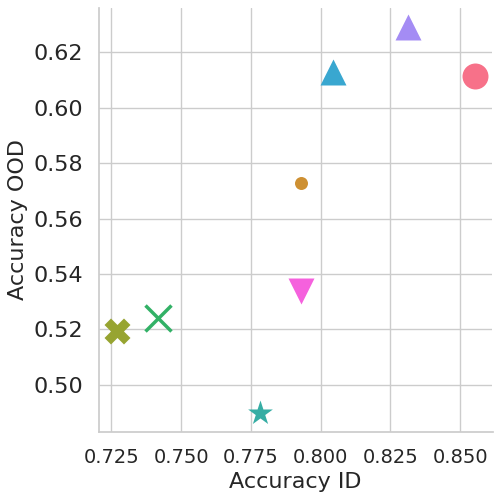
\includegraphics[width=0.27\textwidth]{images/Accuracy ID_KDplot.png}
                                                                                 &
            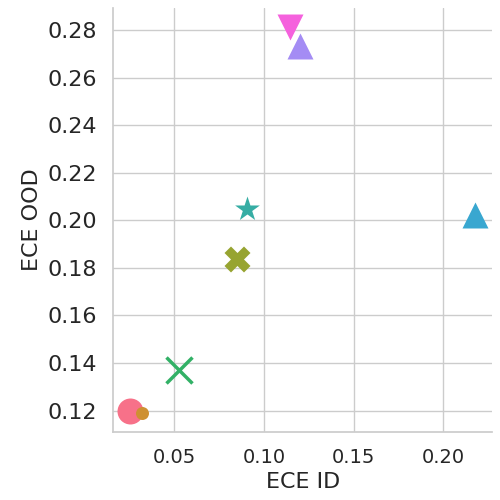
\includegraphics[width=0.27\textwidth]{images/ECE ID_KDplot.png} &
            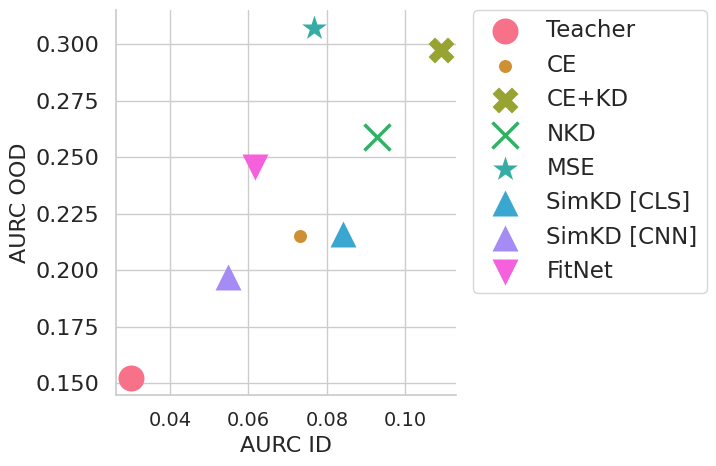
\includegraphics[width=0.42\textwidth]{images/AURC ID_KDplot.png}  \\
        \end{tabular}}
\end{table*}


\paragraph{DIC-KD} This task benchmark reports on experiments with 3 backbones, 2 student architectures (except 1 for Resnet), and 6 KD methods each. \cref{tab:dic} details the ViT and DiT results, whereas the ResNet results (following similar trends) are available in \cref{tab:results_rvl_resnet}.
The same set of experiments was repeated for randomly initialized students (\cref{tab:ablation-vit-rand,tab:ablation-cnn-rand}).
Given the comprehensive scope of the DIC experiments, we can make claims regarding the overall most performant KD method, the teacher-student capacity gap, and the architecture-pretraining gap.
ViT-Small student distilled with the SimKD~\cite{SimKD} method performs best in terms of accuracy and AURC. Note that the best ViT-Tiny student with only 5.5M parameters reaches 83\% accuracy with SimKD, only 2.9\% behind the best ViT-Small student with 86M parameters, showing the potential of advanced KD methods in retaining accuracy at such a large capacity gap.
SimKD performs admirably in terms of accuracy, sometimes (depending on the projector type (MLP and CNN)) as well as the supervised teacher. In terms of AURC, NKD and MSE approaches are best-performing, which are both response-based methods. 
% Another interesting property we investigated has been the pretraining gap by doing distillation experiments from ViT-to-ViT and DiT-to-ViT to see how document pretraining impacts KD performance.
Regarding the pretraining gap, as shown in \cref{tab:dic}, results indicate that a self-supervised teacher like DiT does not meet expectations when distilling the knowledge to a ViT-based student pretrained with ImageNet weights. This could be attributed to the large representation gap in the feature space between the RVL-CDIP pretrained and ImageNet pretrained models. However, evaluation under covariate shift on RVL-CDIP-N, as shown in ~\cref{tab:rvl_n}, demonstrates DiT-based students (distilled with response-based KD strategies) to perform better than ViT$\to$ViT students, pointing to the potential of self-supervision for robust to distribution shift.


% \draft{
% \begin{enumerate}
%   \item Overall most performant method (ranking)
%         \begin{itemize}
%           \item Does the best tiny approximate small?
%           \item SimKD is a particularly strong KD method, always outperforming vanilla KD and supervised student fine-tuning.
%           \item Accuracy: SimKD with either a CNN projector (DiT) or CLS MLP projector (ViT)
%           \item ECE: irrespective of accuracy,
%           \item AURC: NKD and MSE are the highest ranked, although the former does not perform too great in terms of accuracy
%         \end{itemize}
%   \item \textbf{Teacher-student capacity gap}
%         \begin{itemize}
%           \item Does the best tiny approximate small?
%           \item Are some methods better at retaining accuracy at a larger capacity gap?
%         \end{itemize}
%   \item  \textbf{Architecture-pretraining gap}
%         \begin{itemize}
%           \item ViT-to-ViT gives better performance than DiT-to-ViT, which prompts the recommendation to not try to distill from a differently pretrained architecture.
%           \item  Is it better to use a self-supervised closer to ldomain teacher (DiT)?
%                 No, there seems to be a feature representation gap that worsens transfer from a self-supervised teacher to a ViT student pretrained on ImageNet.
%           \item However, evaluation on RVL-CDIP-N does show that DiT-based students (logit-based) are more robust to domain shift than ViT-based students.
%         \end{itemize}
% \end{enumerate}

% Rand observations:   
% \begin{itemize}
%     \item ViT suffer more from student weight initialization, which is evidenced by an average accuracy of 0.5962 for ViT-S/T$_{\operatorname{rand}}$ compared to 0.7675 for R50$_{\operatorname{rand}}$.
%     \item When the student initialization is not dependent on pretraining, NKD pops up as a performant method, showing the versatility of response-based methods when transfer of feature representations is harder.
%   \end{itemize}

% }



\begin{table*}[h]
    \centering
    \caption{Results of KD strategies for D/ViT-B teachers on the \rvl{} dataset.}
    \label{tab:dic}
\begin{minipage}{1\textwidth}
        \npdecimalsign{.}
        \nprounddigits{3}
        \begin{multicols}{2}
            %\centering
            \resizebox{0.53\textwidth}{!}{%
                \begin{tabular}{|r|c|n{1}{3}n{1}{3}n{1}{3}|}
                    \hline
                    \multicolumn{5}{|c|}{ViT-B}                                                                                                                                         \\
                    \hline
                    Student        & Method                                          & \text{ACC}                     & \text{AURC}                    & \text{ECE}                     \\
                    \hline
                    --             & ViT-B                                           & 0.890997274931873              & 0.017270862525174              & 0.033834551278614              \\
                    --             & ViT-S                                           & 0.853371334283357              & 0.02963421682364               & 0.057859288371025              \\
                    --             & ViT-T                                           & 0.822045551138778              & 0.040342312570416              & 0.042795402533132              \\  \hline
                    \textbf{ViT-S} & Vanilla \footnotesize{[$\tau=2.5, \alpha=0.5$]} & 0.85427135678392               & {\npboldmath}0.028376044015258 & {\npboldmath}0.048633268034969 \\
                                   & NKD \footnotesize{[$\tau=1, \gamma=1.5$]}       & 0.840471011775294              & 0.035729143933197              & 0.073632049497662              \\
                                   & MSE                                             & 0.854996374909373              & {\npboldmath}0.028086462460537 & 0.050951811632588              \\
                                   & SimKD \footnotesize{[CLS+MLP]}                  & {\npboldmath}0.85947148678717  & {\npboldmath}0.028154179258953 & 0.28744054887619               \\
                                   & SimKD \footnotesize{[CNN]}                      & 0.846796169904247              & 0.061565487248227              & 0.141136871882953              \\
                                   & FitNet \footnotesize{[middle]}                  & 0.842646066151654              & 0.047789833130271              & 0.140569373835247              \\ \hdashline
                    \textbf{ViT-T} & Vanilla \footnotesize{[$\tau=2.5, \alpha=$]}    & 0.824745618640466              & {\npboldmath}0.03840438493781  & {\npboldmath}0.057973819137046 \\
                                   & NKD \footnotesize{[$\tau=1, \gamma=1.5$]}       & 0.815070376759419              & 0.045976107157128              & 0.093624998224256              \\
                                   & MSE                                             & 0.82329558238956               & 0.039916989542324              & 0.065716418501806              \\
                                   & SimKD \footnotesize{[CLS+MLP]}                  & {\npboldmath}0.829745743643591 & 0.094989035012674              & 0.163239800045468              \\
                                   & SimKD \footnotesize{[CNN]}                      & 0.829495737393435              & 0.055740155161562              & 0.149636502763522              \\
                                   & FitNet \footnotesize{[middle]}                  & 0.812345308632716              & 0.050564425673713              & 0.153136880692877              \\
                    \hline
                \end{tabular}}

            \columnbreak

            %\centering
            \resizebox{0.53\textwidth}{!}{%
                \begin{tabular}{r|c|n{1}{3}n{1}{3}n{1}{3}|}
                    \hline
                    \multicolumn{5}{c|}{DiT-B}                                                                                                                                            \\
                    \hline
                    Student        & Method                                          & \text{ACC}                     & \text{AURC}                    & \text{ECE}                       \\
                    \hline
                    --             & DiT-B                                           & 0.93345                        & 0.07531                        & 0.01036                          \\
                    --             & ViT-S                                           & 0.831345783644591              & 0.041613747046067              & 0.05588416738398                 \\  % weird that it would differ
                    --             & ViT-T                                           & 0.801270031750794              & 0.052664442052395              & 0.047248627795926                \\   \hline
                    \textbf{ViT-S} & Vanilla \footnotesize{[$\tau=2.5, \alpha=0.5$]} & 0.831020775519388              & 0.059765434519678              & 0.07964892708697                 \\
                                   & NKD \footnotesize{[$\tau=1, \gamma=1.5$]}       & 0.7899197479937                & 0.057617085364736              & { \npboldmath} 0.039520166054908 \\
                                   & MSE                                             & 0.831495787394685              & 0.059713971239946              & 0.082210771757924                \\
                                   & SimKD \footnotesize{[CLS+MLP]}                  & 0.838070951773794              & 0.086798506952558              & 0.437770932864024                \\
                                   & SimKD \footnotesize{[CNN]}                      & {\npboldmath}0.850621265531638 & {\npboldmath}0.048178380071352 & 0.135945939814145                \\
                                   & FitNet \footnotesize{[middle]}                  & 0.774894372359309              & 0.062749394618595              & 0.077219594958908                \\   \hdashline
                    \textbf{ViT-T} & Vanilla \footnotesize{[$\tau=2.5, \alpha= $]}   & 0.801195029875747              & 0.063656745246388              & 0.081288359077064                \\
                                   & NKD \footnotesize{[$\tau=1, \gamma=1.5$]}       & 0.771819295482387              & 0.065576326471767              & {\npboldmath}0.041479419489846   \\
                                   & MSE                                             & 0.79534488362209               & 0.076443149642281              & 0.080856397866833                \\
                                   & SimKD \footnotesize{[CLS+MLP]}                  & 0.81609540238506               & 0.104177143748181              & 0.438912200784382                \\
                                   & SimKD \footnotesize{[CNN]}                      & {\npboldmath}0.832270806770169 & {\npboldmath}0.055690336266242 & 0.152081930408472                \\
                                   & FitNet \footnotesize{[middle]}                  & 0.753393834845871              & 0.076718310693334              & 0.053645846570217                \\
                    \hline
                \end{tabular}}
        \end{multicols}
    \end{minipage}
\end{table*}


\paragraph{Covariate shift DIC-KD} To answer if certain KD methods harm a student model's robustness to covariate shift, we plot results per KD method, averaged over the 3 backbones on the (\cref{tab:covarvsid_perKDmethod}).
This re-establishes the superiority of SimKD [CNN] in terms of accuracy, both ID and OOD, yet due to poor calibration, it loses gain on the teacher in terms of AURC. Strikingly, MSE attained the lowest OOD performance, whereas it was a solid ID choice.
\cref{tab:rvl_n} provides more detail on the performance of the different KD methods on RVL-CDIP-N, where we observe that grouped per KD strategy response-based is superior over all metrics.



\section{Conclusion}
KD-based model compression has been a popular technique in recent years, albeit DU research has not paid much attention to efficiency.
Our work explores a limited scope of KD for DU at scale, revealing great potential for creating efficient counterparts of cumbersome DLA models used today.
Moreover, we investigate the potential of DLA for enriching document inputs in downstream DocVQA tasks.
Traditionally, DocVQA has relied on plain OCR text. While structure-preserving OCR provides a notion of geometric layout for downstream, DLA was never considered before for the same purpose, yet our experiments show promise.
The more comprehensive benchmarking of KD methods in DIC with ID evaluation and a covariate shift protocol reveals interesting observations regarding the feature representation and weight initialization gap between DiT (documents) and ViT (natural images), albeit self-supervision for students is more robust in the OOD setting.

%DLA, being capable of region-level class understanding, compels the preprocessed input toward regional modeling for the downstream DocVQA. We find regional modeling to be a valuable and efficient alternative to conventional OCRs for the downstream performance of DocVQA. To this end, looking at the aspect of efficiency, we claim that KD has a fairly high potential for obtaining efficient DLA models. 

% used in preprocessing as it has decent performance for DocVQA with efficient regional modelling.

%While we have explored the scope of KD in the aforementioned context, all the possible KD methods could not covered in this paper and an in-depth analysis of the same would provide a greater understanding of efficiency both at the pre-processing and downstream level. Moreover, multimodal KD was not considered in this work, holding promise to explore more efficient DU models. 
% \jvl{
% Moving toward semantic region-based modeling is a great pursuit, as bootstrapping regions based on more efficient visual document layout models will be key to processing long structured documents in any language-guided application (document editing or question answering, content retrieval).
% Our technical report on model compression with KD methods demonstrates that \todo[inline]{Conclusions from analysis: i) KD has potential for more efficient DLA models, at least when evaluated downstream, ii) .... }
% }

% \jvl{
%   incorporate into above

%   \paragraph{Future work}: The design space of the proposed KD framework is large, and we have only scratched the surface. We believe that the following dimensions are worth exploring:
%   \begin{itemize}
%     \item teachers trained to full convergence are not necessarily the best teachers for feature-based distillation, intermediate teachers might allow for better transfer, as inspired by the information bottleneck theory \cite{tishby2015deep}
% \item  KD methods that are more tailored to the task of DLA, \eg by distilling from intermediate layers of the teacher, or by using a different loss function (\eg contrastive loss)
%     \item classifier-to-detector distillation \cite{guo2021distilling}
% \item cross-architecture KD, \eg from CNN to ViT, or from ViT to CNN
%     \item The breadth of KD methods and approaches: self-distillation [cite], online distillation [cite],
%     \item Building a fully multimodal KD framework also considering document text/OCR inputs and allowing for generative model distillation
% %\item  KD methods that can be used in a meta-architecture like Mask R-CNN, \eg by distilling from the backbone
% \item  KD methods that can be used in a semi-supervised fashion, \eg by distilling from the teacher's unlabeled predictions on the student's unlabeled data
% \item  KD methods that can be used in a multi-task learning setting, \eg by distilling from the teacher's predictions on other tasks
% \end{itemize}
% }


\paragraph{Limitations}
While we primarily use DocLayNet, it remains the DLA dataset with the most diversity in layout elements both in terms of categories and shape or size. However, the downstream DocVQA results urge for more diversity in terms of document types, domains, and objects (\eg layout objects such as logos, watermarks, stamps, signatures, \etc). Thus, the community is in dire need of a dataset diverse enough to guarantee a performance improvement downstream. Moreover, multimodal KD was not considered in this work, holding promise for more efficient, all-round DU models.
The downstream task was not tested on \cite{VanLandeghem2023dude} as multipage documents are more complex to benchmark with limited sequence length LLMs.
Also, DLA being a fairly complicated instance segmentation task, makes it difficult to adapt for KD-based model compression, ruling out some KD methods. This calls for a better experimental framework and architectural modeling to boost the exploration of KD in DLA, in turn, incubating downstream advances in processing and understanding VRDs.

%endcontenthere
{\small
  \bibliographystyle{splncs04}
  \bibliography{main}
}

% WARNING: do not forget to delete the supplementary pages from your submission 
\clearpage
\setcounter{page}{1}


\appendix


\renewcommand{\thesection}{\Alph{section}}
\renewcommand{\thesubsection}{\Alph{section}.\arabic{subsection}}
\crefname{algocf}{alg.}{algs.}
\Crefname{algocf}{Algorithm}{Algorithms}
% \crefalias{section}{appendix}

\section{Code and Datasets}\label{supp:code_and_datasets}

\jvl{
The proposed KD-VDU experimentation framework is available in the Supplementary zip. This includes the DIC benchmarking that is made fully compatible with HuggingFace \textit{transformers}, even allowing arbitrary image classification models and (document) image datasets from HuggingFace \textit{hub}.\\
  The DLA benchmark is built around the \textit{Detectron2} framework, with additional scripts for efficiency evaluation, visualization, and document data preparation for downstream tasks (\Cref{algo:pseudo}).
  Downstream task experiments are made available as a fork of the original LATIN-prompt \cite{wang2023layout} implementations with additional modifications (4-bit quantization, question type ANLS evaluation, InfographicsVQA dataloader, structure-preserving OCR respecting DLA tokens).
}


\section{Implementation Details}\label{supp:implementation_details}

\subsection{DIC}

All runs are documented with hyperparameter configuration and commandline arguments in a \textit{wandb} project that will be released upon acceptance for complete transparency in experiment results and reproducibility. %\href{DistilDoc}{https://wandb.ai/jordy-vlan/DistilDoc}.

For \rvl{}, both teacher and student training is carried out for 10 epochs with a batch size of (32 ViT, 64 ResNet) and AdamW with weight decay 5e-4 and a learning rate of 1e-4 with a linear warmup of 10\%.
For \tobacco{}, the default recipe is similarly trained for 100 epochs. All experiments were performed on a single NVIDIA GeForce RTX 3090 GPU (24GB GPU vRAM).
For some feature-based KD methods, the batch size was necessarily lowered to 16 due to memory constraints.
KD method hyperparameters were cross-validated to find the best performing configuration for each method, and are listed in the main manuscript result tables.

\subsection{DLA}

In this paper, MaskRCNN detection architecture is considered with two different backbones (1) CNNs: ResNet50 and ResNet101 (2) Transformers: ViT base and ViT tiny. All the detection models are trained with Detectron2~\cite{wu2019detectron2} which uses the PyTorch deep learning library. The hyperparameters used are the following: (a) learning rate of 1e-4 (b) iterations 300k (c) optimizer: Adam (d) batch size: 16 (e) ROI heads predictions: 128 (f) NMS threshold: 0.4 (g) confidence threshold: 0.6
% In this paper, two object detection models are considered: (1) Vanilla MaskRCNN: This model is the Mask-RCNN with a ResNet(-50/101) visual backbone. (2) switching to a ViT backbone. We train instance segmentation models with the Detectron2 framework \cite{wu2019detectron2}. Models are trained for 300k iterations with a base learning rate of 1e-4 and a batch size of 512 on a single A40 GPU.
For reproducibility, we share the exact config files used for each experiment as part of the Supplementary,

\paragraph{Teacher and student model variants} \Cref{tab:vistrans,tab:resnet} indicate the differences between used teacher and student models in terms of parameterization and efficiency.

\begin{table}[h]
  \centering
  \caption{Details of Vision Transformer model variants \cite{dosovitskiy2020image}.}
  \scalebox{0.8}{
    \begin{tabular}{l|ccccc}
      \hline \multirow{2}{*}{ Variants } & \multicolumn{5}{|c}{ Settings of D/ViT }                                            \\
                                         & Layers                                   & Width & FFN  & Heads & \#Param           \\
      \hline Tiny (T)                    & 12                                       & 192   & 768  & 3     & $5.5 \mathrm{M}$  \\
      Small (S)                          & 12                                       & 384   & 1536 & 6     & $21.7 \mathrm{M}$ \\
      Base (B)                           & 12                                       & 768   & 3072 & 12    & $85.8 \mathrm{M}$ \\
      %Large (L) & 24 & 1024 & 4096 & 16 & $303.3 \mathrm{M}$ \\
      %Huge (H) & 32 & 1280 & 5120 & 16 & $632 \mathrm{M}$ \\
      \hline
    \end{tabular}}
  \label{tab:vistrans}
\end{table}

\begin{table}[h]
\centering
  \caption{Details of the efficiency of model checkpoints considered in this work.}
  \label{tab:resnet}
\begin{tabular}{llll}
\hline
\textbf{Model}                  & \textbf{GFLOPs} & \textbf{GMACs} & \textbf{Params (M)} \\ \hline
\textit{microsoft/resnet-101  }          & 15.65           & 7.8            & 42.5               \\
\textit{microsoft/resnet-50  }           & 8.21            & 4.09           & 23.51              \\
\textit{google/vit-base-patch16-224}     & 35.15           & 17.56          & 86.39              \\
\textit{microsoft/dit-base }             & 35.15           & 17.56          & 85.81              \\
\textit{WinKawaks/vit-small-patch16-224} & 9.21            & 4.6            & 21.81              \\
\textit{WinKawaks/vit-tiny-patch16-224}  & 2.51            & 1.25           & 5.56            \\ \bottomrule
\end{tabular}
\end{table}



\subsection{Downstream}

We extended the implementation of \cite{wang2023layout} to incorporate Llama-2 \cite{touvron2023llama} and build a similar dataloader for InfographicsVQA \cite{mathew2022infographicvqa}.
To enable strict compatibility, we used the same unified OCR format, DUE \cite{borchmann2021due}, for all datasets. This facilitated easy incorporation of DLA tokens into the OCR tokens without disrupting the logic behind the original layout-aware representation of document text.
As it involved zero-shot evaluation, no finetuning was attempted for this task, and while it could be left for future work, we want to iterate that we sought to explore the innate ability of LLMs to ingest DLA-enriched prompts, and not the downstream task performance itself.


\section{Task definitions}\label{sec:supp-taskdef}

To place each task in the context of document inputs, we define the following tasks and their respective inputs with common notation.
We follow notation established in \cite{van2023beyond} for document page inputs.

A \textbf{page} $p$ consists of an image $\boldsymbol{v} \in \mathbb{R}^{C \times H \times W}$ (number of channels, height, and width, respectively) with $T$ word tokens $u = \left\{w_t\right\}_{t=1}^T$ organized according to a layout structure $s = \left\{\left(x_t^1, y_t^1, x_t^2, y_t^2\right)\right\}_{t=1}^T$, typically referred to as token bounding boxes, coming from OCR or available from a born-digital document.

\subsection{DIC}\label{sec:supp-taskdef_dic}

As a prototypical instance of classification \cite{vapnik1992principles} the goal is to learn an estimator $f: \mathcal{X} \to \mathcal{Y}$ using $N$ supervised input-output pairs $(X,Y) \in \mathcal{X} \times \mathcal{Y}$ drawn \textit{iid} from an unknown joint distribution $P(X,Y)$.
In the context of DIC, the input space $\mathcal{X}$ is the set of all document images, and the output space $\mathcal{Y}$ is the set of all document classes (\eg \textit{invoice, email, form, advertisement}, \etc). The goal is to learn a function $f$ that maps a document image $x \in \mathcal{X}$ to a document class $y \in \mathcal{Y}$, such that $f(x) = y$.
\textit{Covariate shift} \cite{shimodaira2000improving} occurs when the input distribution $P(X)$ changes between the training and evaluation sets, but the conditional distribution $P(Y|X)$ remains the same. Put plainly, both sets share the same document classes, yet the visual appearance, layout and content of the document images can be different. For example, RVL-CDIP \cite{larson2022evaluating} contains more modern documents with color, whereas all \rvl{} documents are greyscale.

\subsection{DLA}\label{sec:supp-taskdef_dla}

The task of DLA can be formulated as a function that processes a document image input and outputs structured information about its logical layout elements (eg. text blocks, headers, figures, charts, plots, tables).
Let  $\mathrm{DLA}(x)$ represent the output predictions of the DLA process as a set of tuples, where each tuple $\left(b_j, c_j, p_j\right)$ represents one of $J$ detected logical layout element.
\begin{equation}
  \mathrm{DLA}(x)=\left\{\left(b_j, c_j, m_j\right)\right\}_{j=1}^J
\end{equation}
For each, $b_j$ denotes the bounding box for the $j$-th detected element, defined as $\left(x_j, y_j, w_j, h_j\right)$ (in the popular COCO format).
$c_j$ is the class label for the $j$-th element, indicating its object category. $m_j$ is a set of additional properties or information (metadata attributes, predicted scores, \textit{considered optional}) associated with the $j$-th element, which can vary depending on the type and context of the layout components.


\subsection{Zero-shot Document Visual Question Answering}\label{sec:supp-taskdef_docvqa}

Given a document $d$ and a question $q$, the goal of zero-shot DocVQA is to predict the answer $a$ to the question $q$ from the document, assuming a single document image for simplicity.
Following the text-only LLM approach in \cite{wang2023layout}, each document image requires to be translated to text, either from OCR or from a born-digital document, and the question is translated to a prompt $p$. The prompt $\boldsymbol{p}$ is a sequence of tokens that is fed to the LLM model, together with a potential task instruction, and the document image text $D$, which is structured following a heuristic procedure operating on the text tokens ($T$) and respective bounding boxes (see \Cref{supp:task_instruction}).

\section{Additional experiment results}\label{sec:supp-results}

\begin{table}[h]
  \centering
  \label{tab:results_rvl_resnet}
  \caption{Results of different KD strategies benchmarked for ResNets applied on the \rvl{} dataset. }
  \npdecimalsign{.}
  \nprounddigits{3}
  \begin{tabular}{|c|c|c|c|n{1}{3}n{1}{3}n{1}{3}|} %{|c|c|c|c||ccc|}  
    \hline Dataset        & Teacher    & Student            & Method                           & \text{ACC}                     & \text{AURC}                    & \text{ECE}                     \\  \hline %$\triangle \mathrm{Acc}$
    \rvl                  & ResNet-101 & --                 & Baseline                         & 0.819445486137153              & 0.042835121898704              & 0.016672567411534              \\
                          & --         & ResNet-50          & Baseline                         & 0.78334                        & 0.05858                        & 0.03865                        \\
\hline \hline \rvlone & ResNet-101 & \textit{ResNet-50} & Vanilla [$\tau=2.5, \alpha=0.5$] & 0.783419585489637              & 0.058696574279648              & 0.039301994115181
    \\
\hline \rvlone        & ResNet-101 &                    & NKD [$\tau=1, \gamma=1.5$]       & 0.784894622365559              & 0.062928657677387              & 0.072927374701675
    \\
\hline \rvlone        & ResNet-101 &                    & MSE                              & 0.7859196479912                & 0.058384636708256              & 0.031505212936942
    \\
\hline \rvlone        & ResNet-101 &                    & SimKD [$\varnothing$ projector]  & 0.76934423360584               & 0.067294064500561              & 0.024556334976757
    \\
\hline \rvlone        & ResNet-101 &                    & SimKD [CNN]                      & {\npboldmath}0.796669916747919 & {\npboldmath}0.052530874137723 & {\npboldmath}0.022517000562448 \\
\hline \rvlone        & ResNet-101 &                    & FitNet [middle]                  & 0.758343958598965              & 0.087305462568872              & 0.177673901604004
    \\
    \hline
  \end{tabular}
\end{table}

%placing it here for layout



\subsection{\tobacco{} results}\label{sec:supp-tobacco}

\begin{table}[h]
    \centering
    \caption{Results of different KD strategies benchmarked for ResNets applied on the \tobacco{} dataset. }
    \npdecimalsign{.}
    \nprounddigits{3}
    \begin{tabular}{|c|c|n{1}{3}n{1}{3}n{1}{3}|} %{|c|c||ccc|}  
        \hline  Student & Method          & \text{ACC}          & \text{ECE}          & \text{AURC}         \\  \hline %$\triangle \mathrm{Acc}$
        --              & Teacher         & 0.4452054794520548  & 0.1023725407268614  & 0.3595245486664192  \\
        ResNet-50       & CE              & 0.5519742143432715  & 0.0962665486513463  & 0.2559003813270729  \\
                        & CE+KD           & 0.6674053182917002  & 0.12730255396398774 & 0.14946885963574724 \\
                        & NKD             & 0.435535858178888   & 0.0760288046947609  & 0.3302691196364132  \\
                        & MSE             & 0.39927477840451253 & 0.08282232649870494 & 0.3785836239288307  \\
                        & SimKD [CLS+MLP] & 0.1764705882352941  & 0.2504398388357339  & 0.7675172798729214  \\
                        & SimKD [CNN]     & 0.314262691377921   & 0.1029121866727384  & 0.4290104103828126  \\
                        & FitNet          & 0.5769540692989524  & 0.0849604828764987  & 0.2191476496623834  \\
        \hline
    \end{tabular}
\end{table}

\begin{table}[h]
    \centering
    \caption{Results of different KD strategies benchmarked for ViT-B applied on the \tobacco{} datasets. }
    \npdecimalsign{.}
    \nprounddigits{3}
    \begin{tabular}{|c|c|n{1}{3}n{1}{3}n{1}{3}|} %{|c|c||ccc|}  
        \hline  Student & Method          & \text{ACC}         & \text{ECE}          & \text{AURC}          \\  \hline %$\triangle \mathrm{Acc}$
                        & Teacher         & 0.8759065269943593 & 0.08187206812541135 & 0.040448066777990316 \\
        ViT-S           & CE              & 0.7832393231265109 & 0.0955075391183256  & 0.0711374806067261   \\
                   & CE+KD           & 0.8140388575521533 & 0.07176496666726945 & 0.0633904758649212   \\
                   & NKD             & 0.8029814665592264 & 0.0938344161588275  & 0.0662325254143168   \\
                   & MSE             & 0.8070104754230459 & 0.1605649162609187  & 0.0618856440822465   \\
                   & SimKD [CNN]     & 0.8360193392425463 & 0.1251863664816119  & 0.0724005793664524   \\
                   & FitNet          & 0.8207091055600322 & 0.1509634972002888  & 0.0588491465898949   \\
        ViT-T            & NKD             & 0.7917002417405318 & 0.0641079216018787  & 0.069245891963159    \\
                    & MSE             & 0.798146655922643  & 0.1984227054859725  & 0.0735070428832557   \\
                    & SimKD [CLS+MLP] & 0.8106365834004835 & 0.5985289354066422  & 0.0648787085907035   \\
                    & SimKD [CNN]     & 0.8098307816277196 & 0.1354849092740382  & 0.0809560984015164   \\
                    & FitNet          & 0.8049959709911362 & 0.1597730596636112  & 0.0699693282483987   \\
        \hline
    \end{tabular}
\end{table}


\begin{table}[h]
    \centering
    \caption{Results of different KD strategies benchmarked for DiT-B applied on the \tobacco{} dataset. }
    \npdecimalsign{.}
    \nprounddigits{3}
    \begin{tabular}{|c|c|n{1}{3}n{1}{3}n{1}{3}|} %{|c|c||ccc|}  
        \hline  Student & Method          & \text{ACC}         & \text{ECE}          & \text{AURC}          \\  \hline %$\triangle \mathrm{Acc}$
                        & Teacher         & 0.9157937147461724 & 0.10934226214285338 & 0.020224875980761052 \\
        ViT-S           & CE              & 0.8203062046736502 & 0.0814063729152479  & 0.0588624099543952   \\
                        & CE+KD           & 0.8247381144238517 & 0.0862504579937333  & 0.0640506857361909   \\
                        & NKD             & 0.8134568896051572 & 0.1005910211374066  & 0.0546015365917559   \\
                        & MSE             & 0.8178887993553586 & 0.0899262672633917  & 0.0628544844656569   \\
                        & SimKD [CLS+MLP] & 0.8287671232876712 & 0.153417345835834   & 0.0564420474488556   \\
                        & SimKD [CNN]     & 0.8102336825141015 & 0.1439121554303226  & 0.0616198570583999   \\
                        & FitNet          & 0.8267526188557615 & 0.1518501442204935  & 0.0672843465750516   \\
        ViT-T           & CE              & 0.8098307816277196 & 0.0661681695247637  & 0.0654695722097237   \\
                        & CE+KD           & 0.8158742949234489 & 0.0783952415517796  & 0.0653438875243606   \\
                        & NKD             & 0.8074133763094279 & 0.0870619831212003  & 0.0627697740360264   \\
                        & MSE             & 0.8110394842868655 & 0.07172337819212    & 0.0612593916183559   \\
                        & SimKD [CLS+MLP] & 0.7784045124899275 & 0.1618730481729019  & 0.0932069554917277   \\
                        & SimKD [CNN]     & 0.7832393231265109 & 0.1871144099522751  & 0.079314938932642    \\
                        & FitNet          & 0.7929089443996776 & 0.1681748113019345  & 0.0765789086236187   \\
        \hline
    \end{tabular}
\end{table}



\subsection{\prima{} results}\label{sec:supp-prima}

\begin{table}[h]
\centering
\caption{Results for DLA-KD experiments on \prima{} dataset.}
\label{res:prima}
\begin{tabular}{@{}cccc@{}}
\toprule
\textbf{Teacher} & \textbf{Student} & \textbf{Method} & \textbf{mAP} \\ \midrule
Vit-B            & -                & Teacher        &         36.01     \\ %interpolated
Resnet-101       & -                & Teacher        & 38.34        \\
-                & ViT-T            & Baseline        &   32.64           \\ %interpolated
-                & Resnet-50        & Baseline        & 35.61        \\
                 &                  &                 &              \\
Resnet-101       & Resnet-50        & SimKD           & 35.00           \\
                 &                  & ReviewKD        & 34.31        \\
Vit-B            & ViT-T            & SimKD           &       32.05      \\ %interpolated
                 &                  & ReviewKD        &     31.94         \\ %interpolated 
                 \bottomrule
\end{tabular}
\end{table}


% Assumption:
% many DLA bboxes (start and end) spread over the whole document, better to iterate over OCR tokens and check DLA bboxes in inner loop
% \# optimization: sort DLA\_pred start and end positions; and insert them in order
% \# give naive implementation here; describe some optimizations and assumptions outside; e.g., sorting to make updates of positions and line ranges easier
% Our proposed algorithm has a time complexity of at least $O(N(M+L))$ and a space complexity of $O(NM)$



\subsection{RVL-CDIP-N results}\label{sec:supp-N}

\begin{table*}[h]
  \centering
  \caption{Evaluation including relative runtime of KD methods on \textit{RVL-CDIP-N}, where from left-to-right results are grouped per KD strategy, per backbone, per student size.}
  \label{tab:rvl_n}
  \begin{tabular}{ccc}
    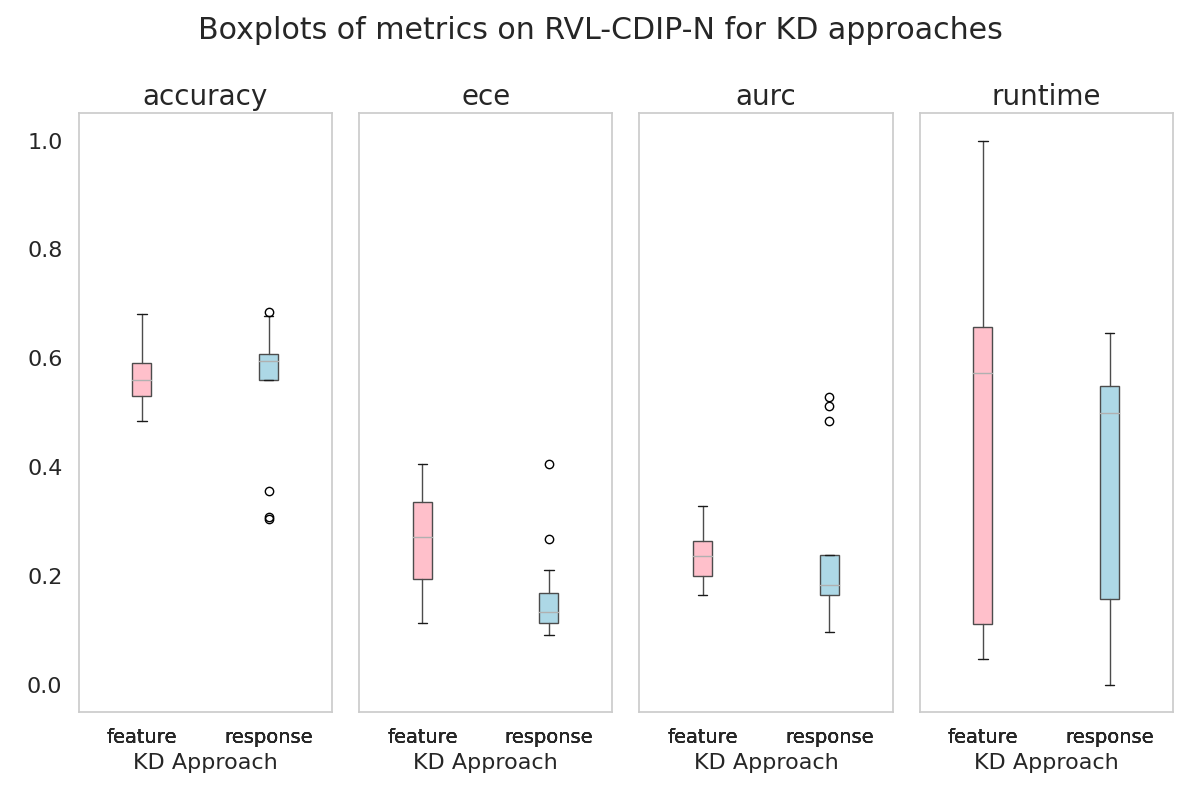
\includegraphics[width=0.33\textwidth]{images/N_results_perKDapproach.png}               &
    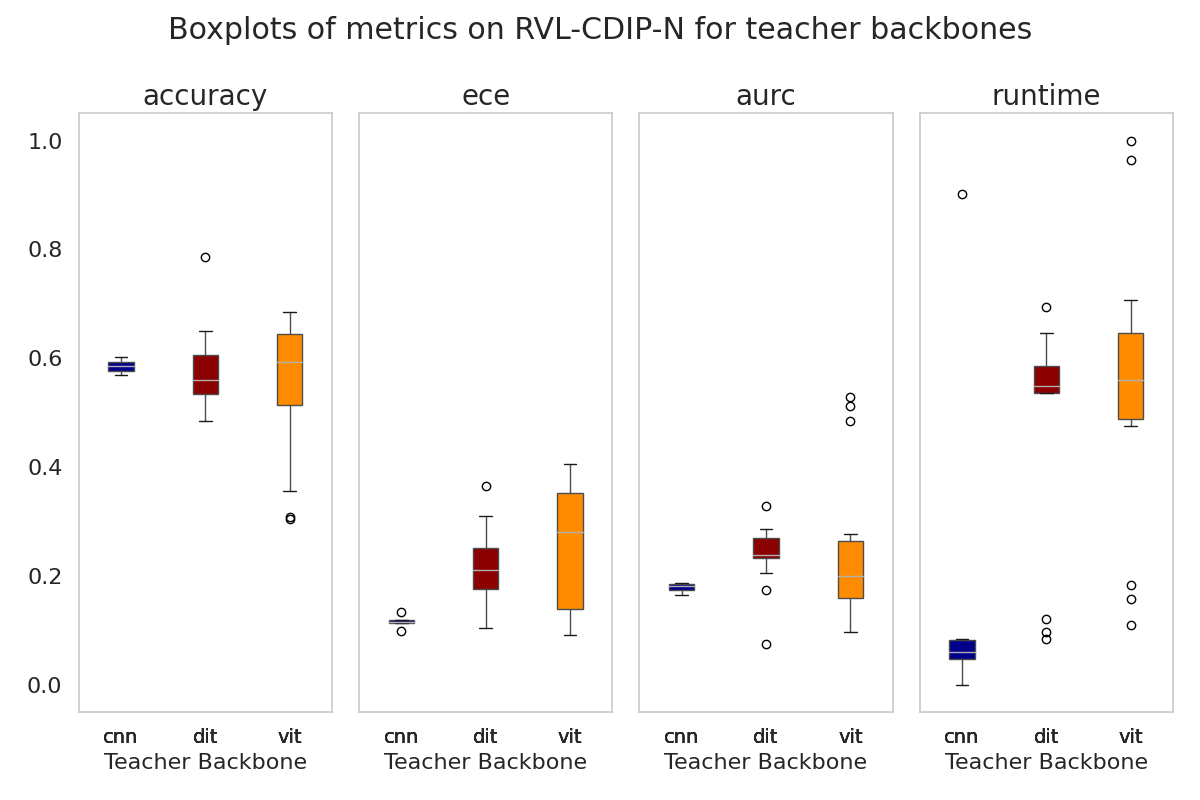
\includegraphics[width=0.33\textwidth]{images/N_results_perbackboneincludingteacher.png} &
    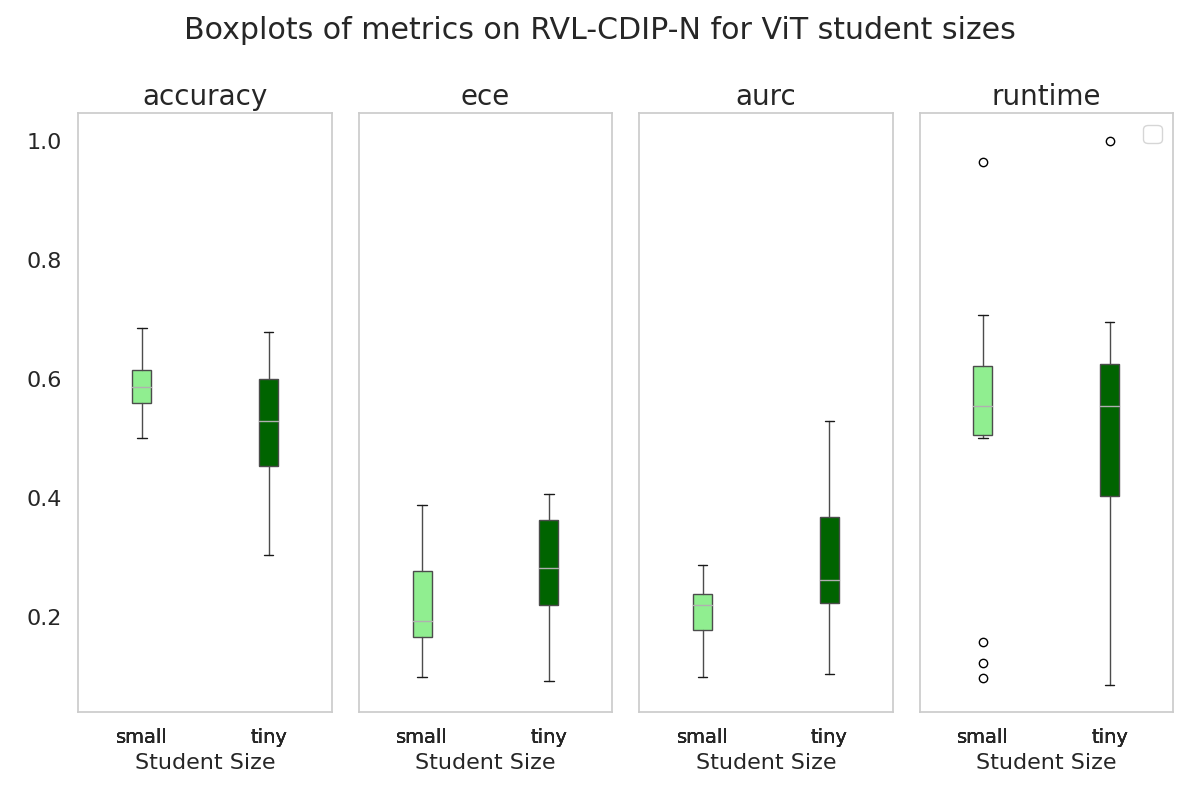
\includegraphics[width=0.33\textwidth]{images/N_results_perstudentsizes.png}               \\
  \end{tabular}
\end{table*}

%averaged
\begin{table}[h]
  \centering
\caption{Results for KD methods when averaged over architectures and student sizes on \textit{RVL-CDIP-N}.}
  \label{tab:N-averaged}
\npdecimalsign{.}
\nprounddigits{3}
\begin{tabular}{|c|n{1}{3}n{1}{3}n{1}{3}|}\toprule
KD method       & \text{ACC}          & \text{ECE}         & \text{AURC}          \\
\toprule
    Teacher         & 0.6112774451097804  & 0.11991748103719505 & 0.15233393563537376 \\
    CE              & 0.5728542914171657  & 0.11916570214335309 & 0.2153090718245799  \\ \hline
    CE+KD           & 0.519294743845642   & 0.18391029421222735 & 0.29761847107836364 \\
    NKD             & 0.5242015968063872  & {\npboldmath}0.1371122426622939  & 0.25916237807196807 \\
    MSE             & 0.49001996007984044 & 0.20466506234305107 & 0.3075089149168292  \\
    SimKD [CLS+MLP] & 0.6129740518962076  & 0.20244919407569956 & 0.21609770922954982 \\
    SimKD [CNN]     & {\npboldmath}0.6291417165668662  & 0.2734916702091337  & {\npboldmath}0.1967929796431719  \\
    FitNet          & 0.5338212463960966  & 0.28147035326753334 & 0.2455269397978257  \\
\bottomrule
  \end{tabular}
\end{table}

\subsection{Downstream DocVQA detail results}

\begin{figure}[h]
  \label{fig:ANLS_mAP_DLAplot}
  
\includegraphics[width=0.5\textwidth]{images/ANLS_DLAplot.png}
\end{figure}

\begin{table*}[h]
  \centering
  \label{tab:detail_dla_downstream_docvqa}
  \caption{Validation \ANLS{} (scaled to \%) of \textsc{Llama-2-7b-chat} \cite{touvron2023llama} on SP-DocVQA \cite{mathew2021docvqa}, with a KD-DLA model enriching the prompt.}
  \resizebox{\columnwidth}{!}{
    \begin{tabular}{@{}ll|c@{\extracolsep{0.25em}}>{\small}c@{\extracolsep{0.25em}}>{\small}c@{\extracolsep{0.25em}}>{\small}c@{\extracolsep{0.25em}}>{\small}c@{\extracolsep{0.25em}}>{\small}c@{\extracolsep{0.25em}}>{\small}c@{\extracolsep{0.25em}}>{\small}c@{\extracolsep{0.25em}}>{\small}c@{\extracolsep{0.25em}}>{\small}c@{}}
      \toprule
      prompt      & DLA                & ANLS  & Image/Photo & Yes/No & Figure/diagram & Form  & Free\_text & Handwritten & Layout & Others & Table/list \\ \midrule
      plain       &                    & 4.3   & 4.25        & 5.36   & 1.46           & 2.69  & 8.99       & 1.74        & 6.1    & 7.72   & 1.87       \\
      space       &                    & 4.61  & 2.97        & 0.0    & 1.25           & 3.31  & 7.55       & 2.14        & 6.48   & 8.45   & 2.59       \\
      task        &                    & 57.63 & 45.38       & 51.52  & 34.97          & 67.88 & 69.71      & 53.19       & 55.51  & 55.78  & 53.81      \\
      +DLA        & Resnet-101         & 57.76 & 43.31       & 47.02  & 35.01          & 66.84 & 70.03      & 52.27       & 57.16  & 58.77  & 52.22      \\
                  & Resnet-101         & 57.55 & 44.44       & 49.4   & 34.0           & 66.99 & 68.64      & 51.97       & 56.52  & 58.23  & 52.64      \\

                  & Resnet-50 ReviewKD & 57.76 & 43.31       & 47.02  & 35.01          & 66.84 & 70.03      & 52.27       & 57.16  & 58.77  & 52.22      \\
                  & Resnet-50 SimKD    & 57.53 & 45.45       & 51.52  & 35.28          & 67.39 & 68.73      & 52.23       & 56.71  & 56.5   & 52.2       \\

                  & Vit-B              & 58.39 & 44.43       & 41.67  & 34.81          & 66.38 & 67.82      & 52.1        & 59.19  & 55.91  & 52.79      \\
                  & Vit-T              & 58.65 & 44.7        & 50.3   & 36.19          & 67.65 & 68.0       & 52.49       & 59.29  & 57.03  & 52.72      \\

                  & Vit-T ReviewKD     & 57.96 & 45.9        & 47.32  & 33.49          & 66.68 & 68.92      & 51.15       & 58.46  & 56.32  & 51.89      \\
                  & Vit-T SimKD        & 58.58 & 45.09       & 49.43  & 34.92          & 67.28 & 70.64      & 52.19       & 58.44  & 57.68  & 52.82      \\
      task\_space &                    & 62.46 & 42.95       & 49.43  & 40.93          & 71.15 & 70.59      & 55.87       & 61.87  & 61.05  & 58.31      \\
      +DLA
                  & Resnet-101         & 61.86 & 41.51       & 48.24  & 40.63          & 71.12 & 69.39      & 54.56       & 61.38  & 58.62  & 57.48      \\
                  & Resnet-50          & 62.08 & 39.62       & 49.13  & 42.4           & 71.27 & 70.37      & 54.43       & 61.54  & 59.86  & 57.59      \\

                  & Resnet-50 ReviewKD & 62.14 & 44.09       & 42.26  & 40.39          & 70.6  & 69.69      & 53.07       & 61.8   & 60.14  & 58.29      \\
                  & Resnet-50 SimKD    & 61.95 & 43.93       & 44.97  & 40.57          & 71.02 & 70.12      & 54.95       & 61.43  & 60.74  & 57.69      \\

                  & Vit-B              & 61.2  & 44.58       & 49.13  & 40.28          & 68.95 & 68.39      & 52.81       & 61.38  & 56.44  & 56.7       \\
              & Vit-T & 58.65 & 44.7 & 50.3 & 36.19 & 67.65 & 68.0 & 52.49 & 59.29 & 57.03 & 52.72  \\ 

                  & Vit-T ReviewKD     & 61.58 & 46.25       & 46.75  & 37.84          & 69.37 & 69.27      & 53.86       & 61.5   & 58.44  & 57.63      \\
                  & Vit-T SimKD        & 61.46 & 44.79       & 48.24  & 40.25          & 69.55 & 69.95      & 53.15       & 61.0   & 58.18  & 57.05      \\
      \bottomrule
    \end{tabular}} %missing = ViT-T
\end{table*}

\begin{table*}[h]
  \centering
  \label{tab:detail_dla_downstream_infographicsvqa}
  \caption{Validation \ANLS{} (scaled to \%) of \textsc{Llama-2-7b-chat} \cite{touvron2023llama} on InfographicsVQA \cite{mathew2022infographicvqa}, with a KD-DLA model enriching the prompt.}

  \resizebox{\columnwidth}{!}{

    \begin{tabular}{@{}ll|c@{\extracolsep{0.25em}}>{\footnotesize}c@{\extracolsep{0.25em}}>{\footnotesize}c@{\extracolsep{0.25em}}>{\footnotesize}c@{\extracolsep{0.25em}}>{\footnotesize}c@{\extracolsep{0.25em}}>{\footnotesize}c@{\extracolsep{0.25em}}>{\footnotesize}c@{\extracolsep{0.25em}}>{\footnotesize}c@{\extracolsep{0.25em}}>{\footnotesize}c@{\extracolsep{0.25em}}>{\footnotesize}c@{\extracolsep{0.25em}}>{\footnotesize}c@{\extracolsep{0.25em}}>{\footnotesize}c@{\extracolsep{0.25em}}>{\footnotesize}c@{}}
      \toprule
      prompt     & DLA            & ANLS  & Arithmetic & Comparison & Counting & Figure & Map   & Multi-span & Non-extractive & Question span & Single span & Table/list & Text  & Visual/layout \\ \midrule
      plain      &                & 0.81  & 0.0        & 0.0        & 0.23     & 0.42   & 0.0   & 0.93       & 0.12           & 0.64          & 0.98        & 1.0        & 1.93  & 0.47          \\
      space      &                & 0.69  & 0.0        & 0.0        & 0.0      & 0.32   & 0.0   & 0.9        & 0.0            & 0.53          & 0.86        & 1.08       & 1.55  & 0.0           \\
      task       &                & 29.08 & 14.15      & 26.94      & 11.35    & 27.52  & 19.1  & 19.79      & 12.79          & 48.44         & 33.79       & 26.17      & 35.24 & 26.39         \\
      +DLA       & Resnet-50      & 27.94 & 14.1       & 26.21      & 10.28    & 26.19  & 20.25 & 17.7       & 12.28          & 45.14         & 32.7        & 24.79      & 34.3  & 26.96         \\
                 & Resnet-101     & 27.86 & 12.12      & 24.96      & 11.35    & 26.32  & 18.82 & 18.32      & 11.93          & 44.81         & 32.62       & 24.51      & 33.89 & 25.94         \\

  & Resnet-50 ReviewKD & 28.16 & 13.33 & 25.81 & 12.05 & 26.39 & 22.11 & 21.06 & 12.93 & 46.95 & 32.42 & 25.02 & 34.18 & 26.86  \\ 
  & Resnet-50 SimKD & 27.65 & 13.79 & 25.78 & 9.95 & 26.16 & 19.53 & 18.78 & 11.97 & 45.95 & 32.17 & 24.31 & 33.8 & 26.31  \\ 

                 & Vit-B          & 28.36 & 14.93      & 29.15      & 7.64     & 27.05  & 19.0  & 19.41      & 11.21          & 46.87         & 33.35       & 25.56      & 34.59 & 26.69         \\
                 & Vit-T          & 28.32 & 15.06      & 28.02      & 9.58     & 27.25  & 19.01 & 17.0       & 11.82          & 45.67         & 33.48       & 25.02      & 34.81 & 28.33         \\
                 & Vit-T ReviewKD & 28.23 & 13.35      & 27.7       & 10.78    & 26.39  & 20.03 & 20.4       & 11.92          & 45.95         & 32.95       & 25.9       & 35.28 & 27.46         \\
                 & Vit-T SimKD    & 28.18 & 14.82      & 26.31      & 9.6      & 26.19  & 18.96 & 18.09      & 12.51          & 45.36         & 32.87       & 24.93      & 34.71 & 30.98         \\
      task+space &                & 27.97 & 9.78       & 25.13      & 6.99     & 25.93  & 21.04 & 22.33      & 8.2            & 43.36         & 33.53       & 25.76      & 35.06 & 27.47         \\
      +DLA       & Resnet-50      & 27.14 & 8.12       & 23.78      & 6.27     & 24.68  & 18.67 & 19.26      & 7.0            & 41.95         & 33.03       & 25.93      & 34.07 & 28.48         \\
                 & Resnet-101     & 28.08 & 9.49       & 24.31      & 8.04     & 25.88  & 19.72 & 21.01      & 8.63           & 41.23         & 33.77       & 25.87      & 35.24 & 28.44         \\
  & Resnet-50 ReviewKD & 28.07 & 9.59 & 24.18 & 8.41 & 25.88 & 18.67 & 21.37 & 9.01 & 42.86 & 33.53 & 26.2 & 35.49 & 27.8  \\ 
  & Resnet-50 SimKD & 27.68 & 9.98 & 24.45 & 7.11 & 25.71 & 20.65 & 20.87 & 8.4 & 43.36 & 33.19 & 25.51 & 34.56 & 27.81  \\ 
                 
                 & Vit-B          & 28.05 & 9.92       & 25.28      & 7.83     & 26.28  & 19.0  & 21.85      & 8.82           & 41.84         & 33.54       & 25.57      & 34.6  & 29.17         \\
                 & Vit-T          & 27.0  & 9.06       & 23.19      & 7.34     & 25.81  & 21.9  & 18.9       & 8.04           & 39.82         & 32.65       & 23.69      & 33.93 & 28.33         \\
                 & Vit-T ReviewKD & 28.47 & 10.89      & 25.9       & 5.42     & 26.8   & 22.23 & 20.59      & 8.28           & 45.67         & 34.24       & 26.44      & 35.81 & 29.14         \\
                 & Vit-T SimKD    & 27.97 & 10.56      & 25.54      & 8.35     & 26.23  & 20.65 & 20.34      & 9.19           & 44.08         & 33.43       & 25.04      & 33.89 & 30.49         \\
      \bottomrule
    \end{tabular}}
\end{table*}


\subsection{Ablation experiments}

The experiments with random student weight initialization (\Cref{tab:ablation-cnn-rand,tab:ablation-vit-rand}) show that ViTs suffer more from student weight initialization, which is evidenced by an average accuracy of 0.5962 for ViT-S/T$_{\operatorname{rand}}$ compared to 0.7675 for R50$_{\operatorname{rand}}$.
When the student initialization is not dependent on pre-training, NKD pops up as a performant method, showing the versatility of response-based methods when transfer of feature representations is harder.

\begin{table*}[h]
  \centering
  \caption{Results of different KD strategies benchmarked for ViT-B teacher with \textbf{randomly} initialized ($\operatorname{rand}$) ViT students applied on the \rvl{} dataset. }
  \label{tab:ablation-vit-rand}
  \npdecimalsign{.}
  \nprounddigits{3}
  \begin{tabular}{|c|c|c|n{1}{3}n{1}{3}n{1}{3}|} %{|c|c|c|c||ccc|}  
    \hline
    Teacher     & Student                       & Method                           & \text{ACC}                      & \text{AURC}                    & \text{ECE}                     \\
    \hline %$\triangle \mathrm{Acc}$
    ViT-B\_rand & --                            & Baseline                         & 0.5402                          & 0.2354                         & 0.07762                        \\
    --          & ViT-$S_{\operatorname{rand}}$ & Vanilla [$\tau=2.5, \alpha=0.5$] & 0.612540313507838               & 0.175294857762794              & 0.220313611855066              \\
    ViT-B       &                               & NKD [$\tau=1, \gamma=1.5$]       & 0.579339483487087               & 0.193249005225908              & {\npboldmath}0.046056065677199 \\
    ViT-B       &                               & MSE                              & 0.625640641016025               & 0.158831615349294              & 0.202600974177652              \\
    ViT-B       &                               & SimKD [CLS+MLP]                  & 0.609090227255681               & 0.181137176233035              & 0.119806758243756              \\
    ViT-B       &                               & SimKD [CNN]                      & {\npboldmath} 0.681217030425761 & 0.181379503732163              & 0.297443627062409              \\
    ViT-B       &                               & FitNet [middle]                  & 0.627665691642291               & {\npboldmath}0.160859389524292 & 0.155333967824325              \\
    ViT-B       & ViT-$T_{\operatorname{rand}}$ & Vanilla [$\tau=2.5, \alpha=$]    & 0.559763994099852               & 0.211508769478741              & 0.141416511926601              \\
    ViT-B       &                               & NKD [$\tau=1, \gamma=1.5$]       & 0.55166379159479                & 0.21515473788689               & {\npboldmath}0.02545063954946  \\
    ViT-B       &                               & MSE                              & 0.5790394759869                 & {\npboldmath}0.198447223890963 & 0.232325413407598              \\
    ViT-B       &                               & SimKD [CLS+MLP]                  & 0.582014550363759               & 0.198973047339166              & 0.195824995889148              \\
    ViT-B       &                               & SimKD [CNN]                      & {\npboldmath}0.662866571664292  & 0.205125367580942              & 0.315795977829891              \\
    ViT-B       &                               & FitNet [middle]                  & 0.569964249106228               & 0.207300502853132              & 0.142680424442589              \\
    \hline
  \end{tabular}
\end{table*}


\begin{table*}[h]
  \centering
  \caption{Results of different KD strategies benchmarked for ResNet-101 teacher with \textbf{randomly} initialized ($\operatorname{rand}$) ResNet-50 students applied on the \rvl{} dataset.}
  \label{tab:ablation-cnn-rand}
  \npdecimalsign{.}
  \nprounddigits{3}
  \begin{tabular}{|c|c|c|n{1}{3}n{1}{3}n{1}{3}|} %{|c|c|c|c||ccc|}  
    \hline
    Teacher    & Student                              & Method                           & \text{ACC}                      & \text{AURC}                     & \text{ECE}                      \\
    \hline %$\triangle \mathrm{Acc}$
    R101\_rand & --                                   & Baseline                                                                                                                               \\
    --         & R50                                  & Baseline                         & 0.768619215480387               & 0.0154005468667318              & 0.0658814569730499              \\
    \hline
    \hline
    R101       & \textbf{R50$_{\operatorname{rand}}$} & Vanilla [$\tau=2.5, \alpha=0.5$] & 0.76014400360009                & {\npboldmath}0.0174754722636533 & 0.0712623406805409              \\
    R101       &                                      & NKD [$\tau=1, \gamma=1.5$]       & 0.7695942398559964              & 0.0510388437926124              & 0.0722681462728383              \\
    R101       &                                      & MSE                              & 0.76494412360309                & 0.0217444527724846              & 0.0676653037230823              \\
    R101       &                                      & SimKD [CLS+MLP]                  & 0.7659941498537464              & 0.0366757247091165              & 0.0678784568625449              \\
    R101       &                                      & SimKD [$\varnothing$ projector]  & {\npboldmath}0.7736693417335433 & 0.0247123270530981              & {\npboldmath}0.0633802504193506 \\
    R101       &                                      & FitNet [middle]                  & 0.760344008600215               & 0.1770233412769938              & 0.0777638551983715              \\
    \hline
  \end{tabular}
\end{table*}





%can arxiv it
\end{document}
